\chapter{基于联邦半监督学习的参与方样本生成方法}
\thispagestyle{others}
\pagestyle{others}
\xiaosi

\section{本章引言}
随着隐私保护法律的日益严格,联邦学习逐渐成为解决多方协作问题的关键技术之一。尤其是在纵向联邦学习(Vertical Federated Learning, VFL)中,多个数据持有方可以在不泄露原始数据的前提下,通过对齐样本的特征协作训练模型。这种方法在多个领域,如金融、医疗等,具有重要的实际应用价值。在VFL中,具有相同样本ID但特征不同的多方加密对齐样本称为联合样本。联合样本集利用来自多方的更多特征帮助机器学习模型训练。VFL要求所有参与方共享足够的联合样本,这在实际应用中往往难以实现。大多数情况下,对齐样本有限,而未对齐的样本却无法有效利用,导致数据利用效率低下。

为了解决因样本对齐不足导致联合样本稀缺的问题,生成联合样本成为一种潜在的解决方案。目前,已有一些基于VFL的样本生成技术。例如,基于生成对抗网络(GANs)的纵向联邦数据生成方法,以及基于马尔可夫随机场(MRFs)\textsuperscript{\cite{MRFs}}的合成表格数据生成框架。尽管这些生成方法能够通过合成样本增加样本的数量,但需要注意的是,机器学习模型的效果不仅仅依赖样本的数量,样本的质量同样至关重要。通过纵向联邦生成方法得到的联合样本通常是合成的虚拟数据,缺乏真实样本的质量保障。特别是在某些参与方样本缺失较为严重时,即使其他方拥有未对齐的额外样本,这些样本也无法有效加入联合样本集,导致可以用于训练的样本数量极为有限,进而影响纵向联邦生成模型的表现。

除了生成联合样本,另一种可能的解决方式是保留其他参与方的未对齐样本,并利用这些样本为缺少样本的参与方生成数据。通过对齐这些未对齐样本和缺失样本,可以有效增加联合样本的数量。这是本文所探讨的核心技术问题之一。当前,已有一些生成方法可用于为样本稀缺的参与方创建样本,诸如基于生成对抗网络(GANs)、自动编码器(AEs)和去噪扩散概率模型(DDPMs)\textsuperscript{\cite{TabDDPM}}等方法。这些方法通过学习潜在数据分布来合成高质量的数据。然而,在纵向联邦学习的场景下,每一方的数据与其他方的数据通常存在一定的相关性。虽然基于深度学习的生成方法在单方数据上能够表现良好,但它们通常忽视了不同参与方之间的数据相关性,未能充分利用多方数据的关系,从而影响生成样本的质量。

针对上述问题,本章提出了一种基于联邦半监督学习的参与方样本生成方法(Participants Sample Generation method based on VFPU-Multitask, FedPSG-PUM),旨在提升在对齐样本有限时VFL的性能。FedPSG-PUM通过估计缺失特征的表示来生成样本。在高相关性的特征上,FedPSG-PUM通过预测未标记样本的伪标签来扩展训练集;而在低相关性的特征上,则采用生成模型或者填补模型合成数据。随后,FedPSG-PUM在这些增强的样本数据上联合训练多个分类器,从而提升整体VFL模型的效果。此外,FedPSG-PUM通过确保各参与方之间不交换原始数据或模型参数,来保护数据隐私,符合联邦学习环境中的安全要求。

本章后续的结构安排为:4.2节对问题进行分析与定义。4.3节系统性地阐述基于联邦半监督学习的参与方样本生成方法框架,并详细介绍  FedPSG-PUM  的执行流程和算法设计。4.4节详细说明实验设计、数据集准备及实验结果分析。最后,4.5节对本章内容进行总结。

\section{问题分析与定义}
考虑一个典型的两方纵向联邦学习(Vertical Federated Learning, VFL)场景,其中涉及两个参与方通过各自独立的特征集进行合作学习,在保证数据隐私和安全的前提下,共同训练一个机器学习模型\textsuperscript{\cite{yang2019federated}}。参与方包括 Party A 和 Party B,其中只有一方拥有标签。首先,Party A 拥有数据集:
\begin{equation}
	\mathcal{D}^A := \{X^A_i\}_{i=1}^{n^A}
\end{equation}
式中,$X^A_i$ 是第 $i$ 个样本的特征向量,$n^A$ 是样本数量。Party A 的数据仅包含特征,不包含标签。接着,Party B 拥有数据集:
\begin{equation}
	\mathcal{D}^B := \{(X^B_i, Y^B_i)\}_{i=1}^{n^B}
\end{equation}
式中,$X^B_i$ 是第 $i$ 个样本的特征向量,$Y^B_i \in \{0,1\}^C$ 是对应的独热编码(one-hot encoding)真实标签,$C$ 表示类别数,$n^B$ 是样本数量。Party B 拥有标签,这在 VFL 中至关重要,因为标签通常用于监督学习任务。然而,Party B 缺乏足够的特征来单独构建一个准确的模型,因此需要利用 Party A 提供的补充特征,如图 \ref{fig:Missing}\subref{MissingTwo} 所示。

需要强调的是,$\mathcal{D}^A$ 和 $\mathcal{D}^B$ 分别由 Party A 和 Party B 私有保存,双方不能互相暴露其数据集。在 VFL 中,Party A 和 Party B 的数据集 $\mathcal{D}^A$ 和 $\mathcal{D}^B$ 包含了不同样本的特征。为了进行联合学习,需要将具有相同身份的样本对齐。假设通过隐私保护的加密实体匹配技术,双方已经完成了样本对齐,得到了对齐样本集:
\begin{equation}
	\mathcal{D}_{al} := \{X^A_{i_{al}}, X^B_{i_{al}}, Y^B_{i_{al}}\}_{i=1}^{n_{al}}
\end{equation}
式中,$n_{al}$ 是对 齐样本的数量。Party A 拥有对齐样本的特征:
\begin{equation}
	\mathcal{D}^A_{al} := \{X^A_{i_{al}}\}_{i=1}^{n_{al}}
\end{equation}
Party B 拥有对齐样本的特征和标签:
\begin{equation}
	\mathcal{D}^B_{al} := \{X^B_{i_{al}}, Y^B_{i_{al}}\}_{i=1}^{n_{al}}
\end{equation}
如果将 $\mathcal{D}^A$ 和 $\mathcal{D}^B$ 连接起来,并使具有相同身份的样本对齐,得到一个如图 \ref{fig:Missing}\subref{MissingTwo} 所示的单一数据集。这个数据集是垂直分割的,每个方拥有该数据集的一个垂直分区(或部分视图),这正是纵向联邦学习一词的由来。然而,两方之间通常只存在有限数量的对齐样本。除了对齐样本外,每个方还拥有一些非对齐样本,即没有来自另一方对应样本的数据。对于 Party A,非对齐样本表示为:
\begin{equation}
	\mathcal{D}^A_{nl} := \{X^A_{i_{nl}}\}_{i=1}^{n^A_{nl}}
\end{equation}
对于 Party B,非对齐样本表示为:
\begin{equation}
	\mathcal{D}^B_{nl} := \{X^B_{i_{nl}}, Y^B_{i_{nl}}\}_{i=1}^{n^B_{nl}}
\end{equation}
从单一表格数据集(见图 \ref{fig:Missing}\subref{MissingTwo})的角度来看,每个方对于另一方的非对齐样本都没有对应的特征(或标签)。将这些特征(或标签)视为“缺失”。图 \ref{fig:Missing}\subref{MissingTwo} 中的各方样本未对齐的情况可以划分为两个图 \ref{fig:Missing}\subref{MissingOne} 所示的情况,对于B方缺失和对于A方缺失。所以,只需解决其中一个问题即可。

\vspace{-0.1cm}
\begin{figure}[h]
	\centering
	\subfigure[]{
		\label{MissingOne}
		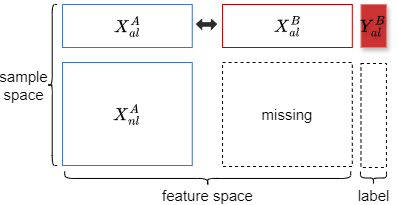
\includegraphics[width=0.45\textwidth]{chapters/imgs/MissingOne}}
	\hspace{0.01\textwidth}  % 适当增加间距
	\subfigure[]{
		\label{MissingTwo}
		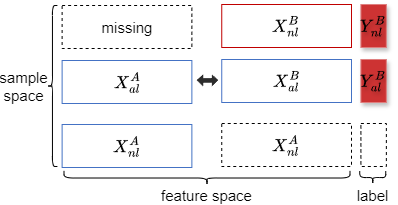
\includegraphics[width=0.45\textwidth]{chapters/imgs/MissingTwo}}
	
	\bicaption[\xiaosi \songti 纵向联邦样本未对齐缺失情况]%
	{\centering \wuhao 纵向联邦样本未对齐缺失情况。(a) B 方缺失情况;(b) 双方缺失情况}%
	{\centering \wuhao Vertical Federated Learning with Unaligned Samples. (a) Missing data in party B; (b) Missing data in both parties}    
	\label{fig:Missing}
\end{figure}
\vspace{-0.35cm}

传统的 VFL 方法仅使用对齐样本 $\mathcal{D}_{al}$ 来构建联邦机器学习模型,而将非对齐样本 $\mathcal{D}^A_{nl}$ 和 $\mathcal{D}^B_{nl}$ 弃置不用。这种做法在对齐样本数量较少时,可能会限制模型的性能,因为大量潜在有用的数据被忽略。

本章提出了一种新的方法  FedPSG-PUM ,旨在充分利用非对齐样本 $\mathcal{D}^A_{nl}$ 和 $\mathcal{D}^B_{nl}$,以提升纵向联邦学习(VFL)模型的性能。该方法结合了 纵向联邦半监督学习 和 表格数据生成技术,通过将对齐样本 $\mathcal{D}_{al}$ 视为有标签数据(其中 $X^A_{al}$ 的“标签”可看作 $X^B_{al}$ 的特征值),而将非对齐样本 $\mathcal{D}^A_{nl}$ 视为无标签数据,利用半监督学习从对齐样本中学习以增强模型的泛化能力,同时采用表格数据生成技术填补与 Party A 相关性较弱的特征缺失值,并与纵向联邦学习相结合优化数据补全。相比传统 VFL 方法, FedPSG-PUM  不仅利用了对齐样本 $\mathcal{D}_{al}$,还充分利用了非对齐样本 $\mathcal{D}^A_{nl}$ 和 $\mathcal{D}^B_{nl}$,显著提高了数据利用率;通过纵向联邦半监督学习,模型能从无标签数据中提取有用信息,进一步提升泛化能力;而表格数据生成技术的引入则使得缺失特征的填补更加合理,从而优化了数据填补策略并提高了模型整体性能。总之, FedPSG-PUM  在传统 VFL 框架基础上引入创新技术,充分利用非对齐样本,在对齐样本有限的情况下显著提升了 VFL 模型的准确性和泛化能力。
\section{基于联邦半监督学习的参与方样本生成方法框架}
如图 \ref{fig: FedPSG-PUM } 所示, FedPSG-PUM  方法的核心包含三个主要流程,这三个流程共同协作以实现跨方数据的高效处理和特征生成。

\vspace{-0.1cm}
\begin{figure}[h]  % 创建一个浮动图形环境,[h]表示尽量将图片放在当前位置(here)
	\centering     % 使图片居中显示
	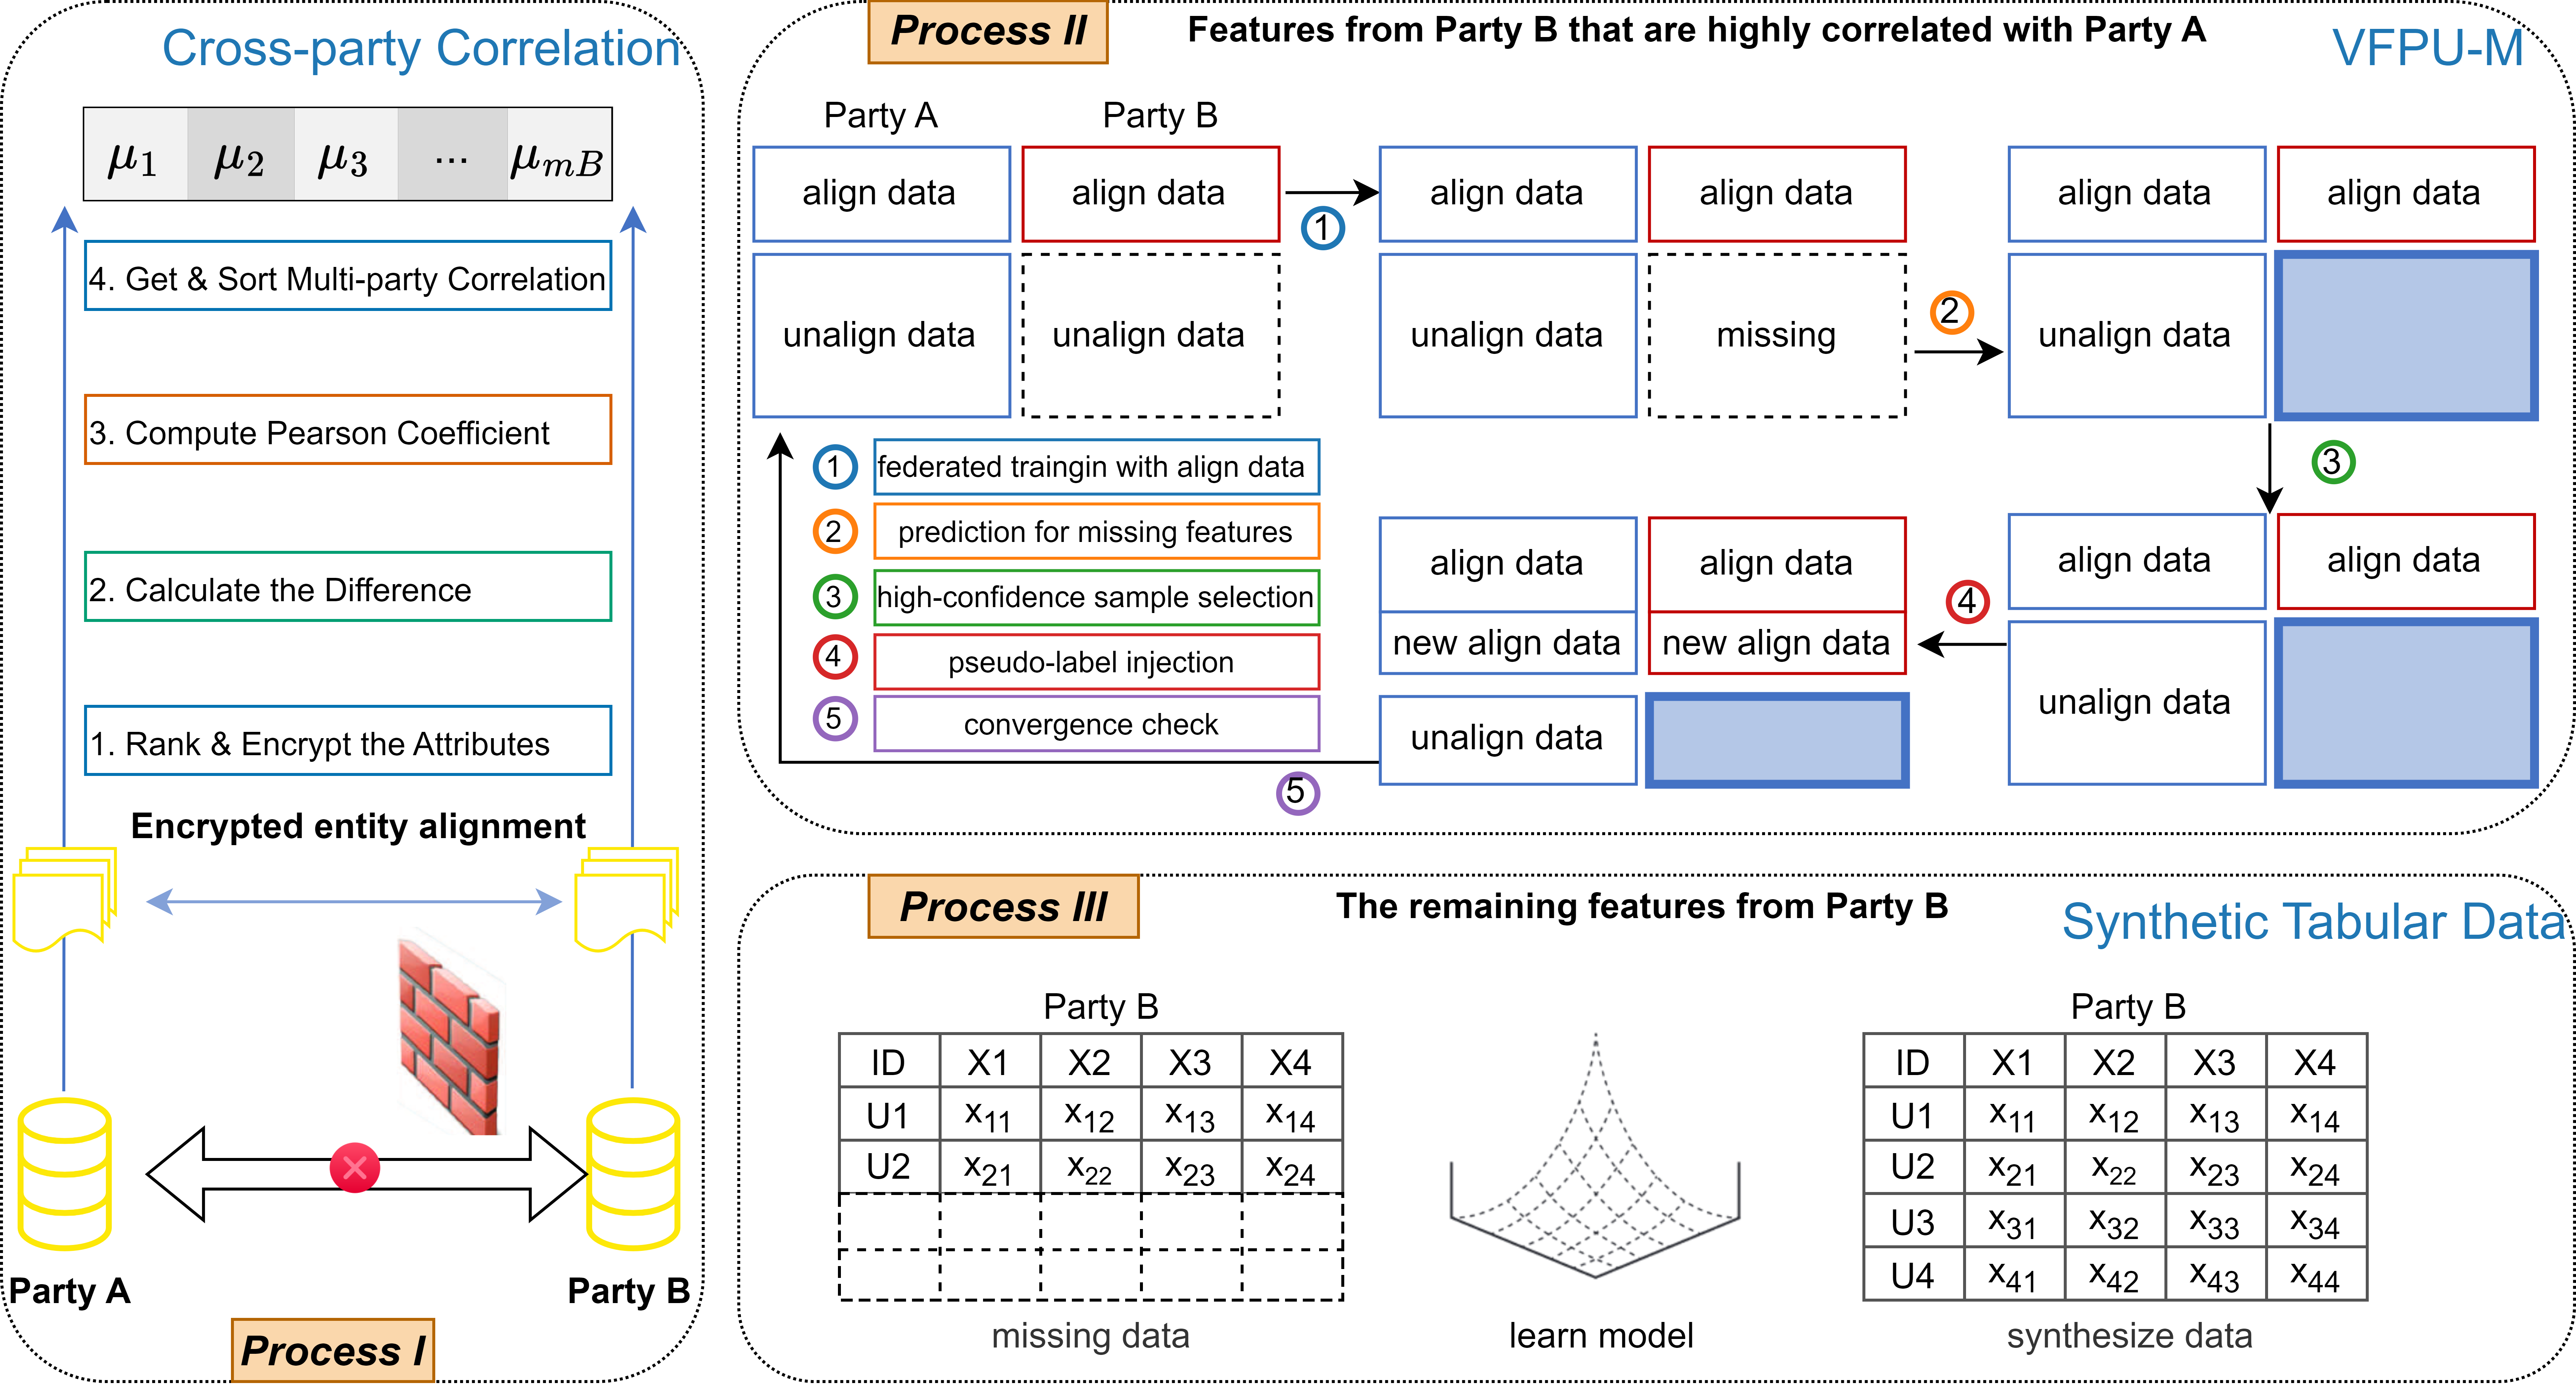
\includegraphics[width=0.9\textwidth]{chapters/imgs/FedPSG-PUM }  
	\bicaption[\xiaosi  FedPSG-PUM 算法总体流程]
	{\wuhao  FedPSG-PUM 算法总体流程}
	{\wuhao The overall process of the proposed  FedPSG-PUM  algorithm}
	\label{fig: FedPSG-PUM }  % 为图片设置标签,可以在文中使用\ref{fig:VFPU}引用此图
\end{figure}
\vspace{-0.35cm}

首先,在 Process I 中,算法通过计算跨方特征之间的相关性,评估和量化各个特征之间的相互依赖关系。这一过程的目标是确保在纵向联邦学习框架中,不同方的特征能够高效对齐,并通过特征相关性分析揭示不同数据源之间可能存在的潜在依赖结构,从而为后续的建模步骤提供更加精确和有针对性的特征信息。接下来,在 Process II 中,方法采用纵向联邦半监督学习算法来进行数据预测。在这一阶段,算法通过结合来自多个方的信息,并利用半监督学习的策略,有效地预测出缺失或未标记的数据。这一过程不仅保证了数据的完整性,还通过有效利用部分标记数据和大量未标记数据,增强了模型的预测能力和鲁棒性。通过这种方式, FedPSG-PUM  方法能够在数据不完全或部分缺失的情况下,依然保持较高的预测精度。最后,在 Process III 中, FedPSG-PUM  方法利用生成模型生成数据。通过对已预测数据和其他相关特征的建模,生成模型能够创造出与真实数据相似的合成数据。这些生成的数据不仅能够补充现有数据的不足,还可以用来进一步优化模型的训练过程,提升模型在实际应用中的泛化能力。生成的数据也有助于应对训练数据中可能出现的偏差或不均衡问题,进一步增强模型的稳定性和可靠性。下面的小节将分别介绍这三个流程。



\subsection{计算跨方特征相关性}
在纵向联邦学习(Vertical Federated Learning, VFL)框架中,不同参与方(Parties)拥有相同样本但不同特征的异构数据。为了有效利用对齐样本的特征信息,需要量化跨参与方特征之间的统计关联性。本节提出了一种基于隐私保护的Spearman秩相关分析方法,用于构建跨方特征相关性排序体系。

设协调方(Coordinator)$ C $ 作为可信第三方,负责生成同态加密(Homomorphic Encryption, HE)密钥对 $ \{\text{pk}, \text{sk}\} $,$ \text{pk} $ 为公钥(Public Key),用于加密数据;$ \text{sk} $ 为私钥(Secret Key),用于解密数据。

协调方 $ C $ 将公钥 $ \text{pk} $ 分发给参与方 A(Party A)和参与方 B(Party B),以便它们对数据进行加密计算,而不直接暴露原始数据,具体计算流程如下:

定义特征列秩向量,设参与方 A 的特征空间为 $X^A \subseteq \mathbb{R}^{m_A}$,$ m_A $ 表示 A 方的特征维数,即 A 方拥有 $ m_A $ 个特征。$ x^A_p \in \mathbb{R}^{n_{al}} $ 表示 A 方第 $ p $ 个特征在对齐样本集 $ \mathcal{D}^A_{al} $ 上的观测向量,$ x^A_p = [x^A_{p1}, x^A_{p2}, ..., x^A_{pn_{al}}] $ 表示该特征在所有对齐样本上的取值,$ n_{al} $ 为对齐样本的数量。

同理,参与方 B 的特征空间为$X^B \subseteq \mathbb{R}^{m_B}$,$ m_B $ 表示 B 方的特征维数,即 B 方拥有 $ m_B $ 个特征。$ x^B_q \in \mathbb{R}^{n_{al}} $ 表示 B 方第 $ q $ 个特征在对齐样本集 $ \mathcal{D}^B_{al} $上的观测向量。$ x^B_q = [x^B_{q1}, x^B_{q2}, ..., x^B_{qn_{al}}] $ 表示该特征在所有对齐样本上的取值,$ n_{al} $ 为对齐样本的数量。

为了计算特征间的相关性,需要首先将特征值转换为秩次。对于任意特征列$x^A_p$,计算其秩向量(Rank Vector):
\begin{equation}
	R^A_p = [r^A_{p1}, r^A_{p2}, ..., r^A_{pn_{al}}]
\end{equation}
式中,$r^A_{pi}$表示样本$i$在特征$x^A_p$上的秩次(Rank),即该样本在该特征列中的排序位置,若存在相同值,则采用平均秩(Average Rank)处理。这种转换可以有效减轻异常值对相关性分析的影响,提高方法的稳健性。类似地,B方的特征列$x^B_q$也可以计算出对应的秩向量:
\begin{equation}
	R^B_q = [r^B_{q1}, r^B_{q2}, ..., r^B_{qn_{al}}]
\end{equation}
基于上述定义,设计了一个安全高效的跨方特征相关性计算流程。首先进行加密秩传输,A方使用公钥$\text{pk}$对秩向量$R^A_p$进行同态加密,得到:
\begin{equation}
	[R^A_p] = \{\text{Enc}(r^A_{p1}), \text{Enc}(r^A_{p2}), ..., \text{Enc}(r^A_{pn_{al}})\}
\end{equation}
并将加密后的秩向量发送给B方。通过同态加密技术,A方可以安全地将自己的特征秩信息分享给B方,而不泄露原始数据。类似地,B方也对自己的秩向量$R^B_q$进行同态加密,得到:
\begin{equation}
	[R^B_q] = \{\text{Enc}(r^B_{q1}), \text{Enc}(r^B_{q2}), ..., \text{Enc}(r^B_{qn_{al}})\}
\end{equation}
接下来进行秩差计算,对于任意特征对$(x^A_p, x^B_q)$,B方计算加密秩差向量:
\begin{equation}
	[D_{pq}] = \left[ \text{Enc}(r^A_{p1} - r^B_{q1}), ..., \text{Enc}(r^A_{pn_{al}} - r^B_{qn_{al}}) \right]
\end{equation}
式中,$d_{pq}^i = r^A_{pi} - r^B_{qi}$表示样本$i$在A方特征$x^A_p$和B方特征$x^B_q$上的秩次之差。这里利用了同态加密的一个重要特性:支持加法运算,使B方可以在加密状态下直接计算秩差,而无需解密原始数据,从而保证了计算过程的隐私安全。计算完成后,B方将加密秩差向量$[D_{pq}]$发送给协调方$C$。在获得加密的秩差向量后,协调方$C$使用私钥$\text{sk}$解密$[D_{pq}]$,得到:
\begin{equation}
	d_{pq}^i = r^A_{pi} - r^B_{qi}, \quad i = 1, ..., n_{al}
\end{equation}
协调方然后基于这些秩差值计算Spearman相关系数,该系数是衡量两个变量单调关系强度的非参数度量:
\begin{equation}
	\rho_{pq} = 1 - \frac{6\sum_{i=1}^{n_{al}} (d_{pq}^i)^2}{n_{al}(n_{al}^2 - 1)}
\end{equation}
式中,$\rho_{pq}$表示A方特征$x^A_p$与B方特征$x^B_q$之间的Spearman相关系数。相较于Pearson相关系数,Spearman相关系数对数据分布不敏感,能够捕获非线性单调关系,更适合异构数据场景。通过计算所有特征对的相关系数,最终可以构建完整的跨方相关性矩阵:
\begin{equation}
	\mathbf{M} \in \mathbb{R}^{m_A \times m_B}, \quad \mathbf{M}(p,q) = \rho_{pq}
\end{equation}
式中,$\mathbf{M}(p,q)$存储A方第$p$个特征列与B方第$q$个特征列的Spearman相关系数,该矩阵全面反映了两方特征空间之间的关联结构。在获得特征间相关性矩阵后,进一步定义特征关联强度的概念。对于B方的每个特征$x^B_q$,计算其与A方所有特征的平均关联强度:
\begin{equation}
	\mu_q = \frac{1}{m_A} \sum_{p=1}^{m_A} \rho_{pq}, \quad q=1,...,m_B
	\label{eq:mu_definition}
\end{equation}

式中,$\mu_q$表示B方特征$x^B_q$对A方特征空间的综合依赖程度。这一指标综合考虑了B方特征与A方所有特征的关联性,可以有效评估该特征在跨方联合建模中的重要程度。关联强度高的特征通常包含更多与对方特征空间相关的信息,在后续的联邦建模中具有更高的价值。最后,基于特征关联强度生成排序列表。具体而言,构建特征重要性序列:
\begin{equation}
	\mathcal{L}_B = \{(\mu_q, \mathbf{x}^B_q)\}_{q=1}^{m_B}
\end{equation}
\subsection{纵向联邦半监督方法预测数据}
如图 \ref{fig: FedPSG-PUM} 所示,在完成跨方相关性矩阵计算后,研究工作进入Process II阶段。这一阶段的核心目标是从B方数据中识别并提取与A方具有较高相关性的特征列,作为数据生成的关键基础。这种特征选择过程绝非随机筛选,而是基于前一阶段通过严格数学建模计算得到的跨方相关性矩阵$\mathbf{M} \in \mathbb{R}^{m_A \times m_B}$,其中$\mathbf{M}(p,q) = \rho_{pq}$存储了A方第$p$个特征与B方第$q$个特征之间的Spearman相关系数。这一矩阵全面量化了双方特征空间之间的统计关联结构,为特征选择提供了可靠的数学依据。

在Process II阶段,特征列的选择遵循一个基于阈值的数学判定准则:系统仅保留那些综合相关强度$\mu_q$超过预设阈值$\tau$的B方特征列。其中,$\mu_q$定义为B方第$q$个特征与A方所有特征的平均相关系数,如公式~\eqref{eq:mu_definition}所示。

这一指标综合评估了B方特征$x^B_q$与整个A方特征空间的统计依赖程度,为后续的纵向联邦半监督学习奠定了理论基础。通过这种基于数学模型的特征筛选机制,系统能够最大限度地保留和利用跨方数据间的内在关联,从而显著提高生成过程的准确性和效率。

\subsubsection{联邦半监督学习框架设计}
在FedPSG-PUM方法中,采用"列级特征分解"(Column-wise Feature Decomposition, CFD)策略,将B方的高相关性特征空间$X^B_{high}$进行分解,使每一列特征$x^B_q$都被单独处理为一个独立的预测目标(即标签列),这种处理方式使得原来数据生成问题,变成某一列的联邦半监督预测问题。

从数学角度看,方法最终试图建立一个多对多的映射函数$f: \mathbb{R}^{d_A} \rightarrow \mathbb{R}^{d_B}$,直接从A方特征空间映射到B方整个特征空间,CFD策略将这一复杂映射分解为$d_B'$个独立的单维映射函数:$f_q: \mathbb{R}^{d_A} \rightarrow \mathbb{R}, q = 1, 2, ..., d_B'$,式中$d_B'$是筛选后的高相关性特征数量($d_B' = |X^B_{high}| \leq d_B$)。每个$f_q$只负责预测一个B方特征,而这个问题可以借助第3章的方法进行解决。

在这一框架下,处理的是以下数据实体:
A方的特征矩阵$X^A \in \mathbb{R}^{n \times d_A}$,式中$n = n_{al} + n_{nl}$表示A方样本总数(对齐和非对齐样本之和),$d_A$表示A方特征维度; B方的对齐特征矩阵$X^B_{al} \in \mathbb{R}^{n_{al} \times d_B}$,式中$n_{al}$表示对齐样本数量,$d_B$表示B方特征维度;待预测的B方非对齐特征矩阵$X^B_{predict} \in \mathbb{R}^{n_{nl} \times d_B'}$,式中$n_{nl}$表示非对齐样本数量,$d_B'$表示高相关性特征数量

对于具体的特征预测过程,采用“多列对一列模型”(Multi-Column-One-Model, MCOM)的策略。对于每个高相关性特征$x^B_q \in X^B_{high}$,单独构建一个联邦半监督学习模型$\mathcal{F}_q$,形式化地:

\begin{equation}
	\mathcal{F}_q: X^A \rightarrow x^B_q, \quad \forall x^B_q \in X^B_{high}
\end{equation}


这种框架设计在多个方面展现出显著优势。首先,采用单特征预测模型能够有效降低模型的参数复杂度,相较于多特征联合建模而言,其过拟合风险更低,泛化能力更强。其次,为每个特征量身定制专属模型,有助于更精准地捕捉其与A方特征空间之间的特定关联模式,从而提升预测精度。此外,不同特征对应的模型可以并行进行训练与推理,显著提高了整体计算效率。在系统鲁棒性方面,该策略也表现出更高的容错性,即便某个模型出现故障,也仅影响对应特征的预测结果,不会导致整个系统失效。更重要的是,该方法具备高度的结构灵活性,能够根据特征的数据类型(如连续值、类别值、有序值等)选择最适合的模型结构进行建模。在CFD策略下,特征 $x^B_q \in \mathbb{R}^{n_{al}}$ 不再仅仅是一个被动的数据属性,而是被赋予了新的角色——在 $X^A$ 与 $X^{B_{predict}}$ 进行纵向联邦学习的过程中,它作为目标预测变量参与建模。这种概念上的重新定义,将特征预测问题巧妙转化为一系列半监督学习任务,不仅能够充分利用现有的半监督学习理论与算法,还能在整个过程中保持对数据隐私的严格保护,契合联邦学习框架的核心要求。

这种多层次的隐私保护架构确保了在整个联邦半监督学习过程中,A方无法访问B方的特征数据$X^B$,B方也无法获取A方的特征数据$X^A$。双方仅通过安全的加密通信渠道交换经过处理的中间结果,如加密梯度、噪声化参数更新等,而非原始数据本身。

协作训练机制的完整数学表达可概括为:A方利用自身数据$X^A$作为输入特征,将B方对齐样本特征$x^B_q|_{al} \in \mathbb{R}^{n_{al}}$作为标签,训练预测模型$\mathcal{M}_q$。训练完成后,A方可对其未对齐样本应用模型,生成预测结果$\hat{x}^B_q|_{nl} \in \mathbb{R}^{n_{nl}}$。最终,对所有高相关性特征重复此过程,可得到完整的B方预测特征矩阵:

\begin{equation}
	X^{B_{predict}} = [\hat{x}^B_1|_{nl}, \hat{x}^B_2|_{nl}, ..., \hat{x}^B_{d_B'}|_{nl}] \in \mathbb{R}^{n_{nl} \times d_B'}
\end{equation}

这种“多列对一列模型”的策略不仅显著提升了预测精度,而且具有很强的可解释性和灵活性,特别适合处理异构数据源之间的特征预测任务。

本文创新性地将纵向联邦学习环境中的数据缺失问题重新形式化为纵向联邦半监督学习框架(Vertical Federated Semi-Supervised Learning, VFSSL)下的多任务预测问题。这种重新建模不仅为解决原问题提供了新的技术路径,还建立了联邦学习与半监督学习的理论桥梁,使两个领域的技术优势得以有效融合。

在数学形式上,考虑A方特征集$X^A \in \mathbb{R}^{n \times d_A}$,式中包含$n = n_{al} + n_{nl}$个样本,每个样本具有$d_A$维特征。这些样本可进一步划分为两个互斥子集:

(1) 有标签子集 $X^A_{L} = X^A_{al} \in \mathbb{R}^{n_{al} \times d_A}$:这部分样本能够与B方样本通过安全实体对齐技术匹配,因此对应的B方特征值$x^B_q|_{al} \in \mathbb{R}^{n_{al}}$是已知的,可作为监督信号(标签)

(2) 无标签子集 $X^A_{U} = X^A_{nl} \in \mathbb{R}^{n_{nl} \times d_A}$:这部分样本没有对应的B方匹配样本,因此缺乏相应的特征标签,需要通过半监督学习技术进行预测

通过这种形式化表达,将问题变换为:对于每个高相关性特征$x^B_q \in X^B_{high}$,构建有标签数据集$\mathcal{D}_L^q$和无标签数据集$\mathcal{D}_U$:
\begin{equation}
	\begin{split}
		\mathcal{D}_{L}^{q} &= \{(x_{i}^{A},y_{i}^{q})|x_{i}^{A}\in X_{L}^{A},y_{i}^{q}=x_{q}^{B}(i),i=1,2,...,{{n}_{al}}\} \\
		{{\mathcal{D}}}_{U} &= \{x_{j}^{A}|x_{j}^{A}\in X_{U}^{A},j=1,2,...,{{n}_{nl}}\}
	\end{split}
\end{equation}
式中,$y_i^q$是B方第$q$个特征在第$i$个对齐样本上的取值,可根据特征类型表现为连续值(回归任务)或离散值(分类任务)。研究目标是学习一组预测函数$\{f_q | q = 1,2,...,d_B'\}$,使得对于任意$x^A \in \mathbb{R}^{d_A}$,$f_q(x^A)$能够准确预测对应的$x^B_q$值。B方特征$x^B_q$可能是连续值(如年龄、收入等)、二分类值(如是/否)或多分类值(如教育水平等),需要算法能够灵活处理不同类型的预测任务。

\subsubsection{多任务联邦半监督学习算法}
根据上述框架设计,本文创新性地提出了改进型VFPU-M(Multi-task VFPU)方法。该方法通过纵向联邦协同训练构建特征预测模型,同时采用伪标签技术有效利用无标签数据,实现了在联邦环境下的高效半监督学习。VFPU-M的核心理念是通过迭代式地提高模型性能并从无标签数据中筛选出高可信度样本,逐步扩展训练集规模,从而在保护隐私的前提下提升预测精度。

\vspace{-0.1cm} 
\begin{table}[h]
	\renewcommand{\arraystretch}{0.6}
	\centering
	{\songti \wuhao
		\begin{tabular}{p{\textwidth}}
			\toprule[1.5pt]
			\makecell[l]{\songti\wuhao  算法 4-1 纵向联邦半监督方法生成数据算法}\\
			\midrule[0.75pt]
			\makecell[l]{\wuhao \textbf{输入:} A方对齐数据集 $X_{al}^A$, 未标记数据集 $X_{nl}^A$,B 方特性相关性列表 $\mathcal{L}_B$}\\
			\makecell[l]{\wuhao \quad 对齐数据集样本数量 $n_{al}$,标记数据集的样本数量 $n_{nl}$,相关性阈值 $\tau$}\\
			\makecell[l]{\wuhao \textbf{输出:} $X^{B_{predict}}$: 最终通过预测方法生成的B方数据}\\
			\makecell[l]{\wuhao \textbf{Process:}}\\
			\makecell[l]{\wuhao 1: Initialize $X^{B_{predict}} = \emptyset$, $\mathcal{L}_B^{\text{predict}} = \{(\mu_q, x^B_q) \in \mathcal{L}_B \mid u_q > \tau\}$}\\
			\makecell[l]{\wuhao 2: \textbf{for} $(\mu_q, x^B_q) \in \mathcal{L}_B^{\text{predict}}$ \textbf{do}}\\
			\makecell[l]{\wuhao 3: \quad $X_{al}^{B_{predict}} = \{x_{i}^{B_{predict}}\}_{i=1}^{n_{al}}$}\\
			\makecell[l]{\wuhao 4: \quad $X_{nl}^{B_{predict}} = \{x_{i}^{B_{predict}}\}_{i=n_{al}+1}^{n_{al}+n_{nl}}$}\\
			\makecell[l]{\wuhao 5: \quad $p = \text{VFPU-M}(X_{al}^A, X_{nl}^A, X_{al}^{B_{predict}}, X_{nl}^{B_{predict}}, x^B_q)$}\\
			\makecell[l]{\wuhao 6: \quad $X^{B_{predict}} = X^{B_{predict}} \cup \{p\}$}\\
			\makecell[l]{\wuhao 7: \textbf{end for}}\\
			\makecell[l]{\wuhao 8: 得到 $X^{B_{predict}}$}\\
			\bottomrule[1.5pt]
		\end{tabular}
	}
	\label{tab:algo-vfpu}
\end{table}
\vspace{-0.35cm}



算法4-1和算法4-2是VFPU-M方法的具体实现,共同构成了我们提出的纵向联邦半监督预测数据的完整技术路线。下面将系统地解析这两个算法的数学原理和实现细节。

(1) 算法4-1:纵向联邦半监督方法生成数据算法

算法4-1提出了一种基于纵向联邦半监督学习的缺失数据生成方法,通过深入挖掘参与方A与B之间对齐样本的统计关联特性,在联邦学习框架下构建特征补全模型,实现在保护各方数据隐私的前提下,高效补全B方未对齐样本的缺失特征。该算法的输入参数包括:A方对齐数据:$X_{al}^A \in \mathbb{R}^{n_{al} \times d_A}$,表示A方与B方样本空间对齐的特征矩阵。这一数据集是算法的核心训练资源,其中$n_{al}$为对齐样本的数量,反映了可用的标记数据规模;$d_A$为A方特征维度,表征了特征空间的复杂度;A方未对齐数据:$X_{nl}^A \in \mathbb{R}^{n_{nl} \times d_A}$,表示A方未对齐部分的特征矩阵。这些样本缺少对应的B方特征标记,是算法需要为其预测B方特征的目标数据集。参数$n_{nl}$为未对齐样本的数量,通常远大于$n_{al}$,表明了无标签数据的丰富程度;B方相关系数列表:$\mathcal{L}_B = \{(\mu_q, X^B_q)\}_{q=1}^{d_B}$,其中$\mu_q$表示B方特征列$X^B_q$与A方数据的综合相关系数(在前文中已定义)。这一列表对B方的每个特征进行了相关性量化,为特征选择提供了理论依据。参数$d_B$为B方特征维度,反映了需要生成的特征空间规模;相关性阈值:$\tau \in [0, 1]$,用于筛选与A方数据具有显著相关性的B方特征列。该阈值的选择直接影响算法的执行路径和生成数据的质量。较高的$\tau$值意味着更严格的特征筛选标准,通常会减少被选择的特征数量,但提高预测的准确性;较低的$\tau$值则会保留更多特征,可能增加噪声但提高了特征覆盖率。该算法的步骤如下:

步骤1:初始化与相关性筛选

算法首先将目标数据集$X^{B_{predict}}$初始化为空集,表示尚未生成任何B方数据:
\begin{equation}
	X^{B_{predict}} = \emptyset
\end{equation}
随后通过相关性筛选,从$\mathcal{L}_B$中选取所有相关性系数大于阈值$\tau$的特征列,构造预测特征集合:

\begin{equation}
	\mathcal{L}_B^{\text{predict}} = \{(\mu_q, X^B_q) \in \mathcal{L}_B \mid \mu_q > \tau\}
\end{equation}

这一筛选过程实质上是一种基于统计显著性的特征选择(Feature Selection)操作,确保只有那些与A方数据有足够强相关关系的B方特征被纳入预测范围。这种策略不仅降低了计算复杂度,而且通过过滤低相关特征减少了噪声干扰,提高了后续预测的准确性。从信息论角度看,筛选过程可以理解为保留了互信息(Mutual Information)较高的特征对,最大化了跨方数据之间的信息传递效率。

相关性阈值$\tau$的选择不是任意的,而是基于数据特性和任务需求的统计量。在实际应用中,可以通过假设检验方法确定统计显著性的$\tau$值,或通过交叉验证等方法从一系列候选值中选择最优$\tau$。不同的$\tau$取值会导致$\mathcal{L}_B^{\text{predict}}$包含不同数量的特征,从而影响算法的执行效率和预测精度。

步骤2:特征级联邦数据生成

算法接下来对每个满足相关性筛选条件的特征列$(\mu_q, X^B_q) \in \mathcal{L}_B^{\text{predict}}$执行迭代预测,这对应伪代码中的循环结构(2-7行)。

对于每个特征列,算法首先进行数据分区操作,将B方特征列$X^B_q$的预测数据划分为两部分:

对齐部分:$X_{al}^{B_{predict}} = \{x_{i}^{B_{predict}}\}_{i=1}^{n_{al}} \in \mathbb{R}^{n_{al}}$,对应于A方对齐样本的B方特征值。这部分数据在B方是已知的,可以直接用于模型训练的标签。

未对齐部分:$X_{nl}^{B_{predict}} = \{x_{i}^{B_{predict}}\}_{i=n_{al}+1}^{n_{al}+n_{nl}} \in \mathbb{R}^{n_{nl}}$,需要通过联邦学习方法进行预测。这部分是算法的预测目标。

这种数据分区方式与A方数据结构$\{X_{al}^A, X_{nl}^A\}$保持一致,确保了后续联邦建模过程中样本索引的对应关系,便于模型学习样本间的映射规律。在实现层面,这种一致性设计简化了代码架构,提高了系统的可维护性和扩展性。

随后,算法调用VFPU-M方法进行联邦预测建模,这是算法的核心功能调用:

\begin{equation}
	p = \text{VFPU-M}(X_{al}^A, X_{nl}^A, X_{al}^{B_{predict}}, X_{nl}^{B_{predict}}, X^B_q)
\end{equation}

在这个函数调用中:$X_{al}^A$和$X_{nl}^A$是A方的对齐和非对齐特征数据,作为预测模型的输入特征;$X_{al}^{B_{predict}}$是B方已知的特征值,作为训练模型的标签;$X_{nl}^{B_{predict}}$是需要预测的B方未对齐特征,在函数调用时可能为空值或初始化值,但会在函数执行过程中被填充为预测结果;$X^B_q$是当前处理的B方特征列,提供了预测任务的目标信息。

VFPU-M函数返回的$p$是预测结果向量,即对$X_{nl}^{B_{predict}}$的估计值。这个预测过程实现了从A方特征空间到B方单个特征的映射学习,是算法的核心预测环节。

步骤3:数据合成与迭代构建

获得预测结果向量$p$后,算法将其合并至目标数据集$X^{B_{predict}}$:

\begin{equation}
	X^{B_{predict}} = X^{B_{predict}} \cup \{p\}
\end{equation}

这一操作逐列构建了B方预测数据矩阵,每次迭代都增加一个新的特征列,直到所有满足相关性条件的特征都被预测完毕。这种逐列构建的策略使得算法能够针对每个特征的特性采用最适合的预测模型,而不是使用一个通用模型预测所有特征,从而提高了预测精度。

通过完整的特征迭代过程,算法最终生成完整的B方预测数据矩阵:

\begin{equation}
	X^{B_{predict}} \in \mathbb{R}^{(n_{al}+n_{nl}) \times |\mathcal{L}_B^{\text{predict}}|}
\end{equation}

其中$|\mathcal{L}_B^{\text{predict}}|$表示通过相关性筛选的B方特征数量。这个矩阵不仅保留了与A方数据的统计相关性,同时也符合纵向联邦学习的隐私保护约束,可以有效地补充B方的缺失数据,扩大可用的联合样本规模。

(2) 算法4-2:VFPU-M算法

算法4-2详细阐述了VFPU-M(Vertical Federated Positive-Unlabeled Learning with Multi-task)算法的实现过程。这是一种面向半监督联邦学习的创新方法,通过迭代伪标签生成和模型更新,实现对无标签数据的高效利用。该算法的输入参数包括:A方数据:$X_{al}^A \in \mathbb{R}^{n_{al} \times d_A}$和$X_{nl}^A \in \mathbb{R}^{n_{nl} \times d_A}$,分别表示A方的对齐和非对齐特征数据;B方数据:$X_{al}^B \in \mathbb{R}^{n_{al}}$和$X_{nl}^B \in \mathbb{R}^{n_{nl}}$,分别表示B方的对齐特征值和需要预测的非对齐特征;标签向量:$y \in \mathbb{R}^{n_{al}}$或$y \in \{0,1,2,...,C-1\}^{n_{al}}$,表示对齐样本的真实标签,可能是连续值(回归任务)或离散类别(分类任务);置信度阈值:$\alpha \in [0,1]$,用于筛选高置信度预测结果,控制伪标签的质量;迭代次数:$T \in \mathbb{N}^+$,算法执行的最大迭代轮数。;选取比例:$k \in (0,1]$,每轮从高置信度样本中选取的比例,用于控制伪标签样本的增长速度。该算法的执行步骤如下:

\vspace{-0.2cm}
\begin{table}[h]
	\centering
	\renewcommand{\arraystretch}{0.6}
	{\songti \wuhao
		\begin{tabular}{p{\textwidth}}
			\toprule[1.5pt]
			\makecell[l]{\songti\wuhao 算法 4-2 VFPU-M 算法} \\
			\midrule[0.5pt]
			\makecell[l]{\wuhao \textbf{输入:} $X_{al}^A$, $X_{nl}^A$: 参与方A的对齐/非对齐数据; $X_{al}^B$, $X_{nl}^B$: 参与方B的对齐/非对齐数据; } \\
			\makecell[l]{\wuhao \qquad $y$: 标签; $\alpha$: 置信度阈值; $T$: 迭代次数; $k$: 选取比例} \\
			\makecell[l]{\wuhao \textbf{输出:} $\mathbf{y}^{\text{pseudo}}$} \\
			\makecell[l]{\wuhao 1: $\mathcal{D}_{L}^{(0)} = \{X_{al}^A, X_{al}^B, y\}$, 
				$\mathcal{D}_{U}^{(0)} = \{X_{nl}^A, X_{nl}^B\}$} \\
			\makecell[l]{\wuhao 2: \textbf{for} $t = 1$ \textbf{to} $T$ \textbf{do}} \\
			\makecell[l]{\wuhao 3: \quad $\theta^{(t)} \leftarrow \arg\min_\theta \sum_{(\mathbf{x}^A,\mathbf{x}^B,y)\in\mathcal{D}_L^{(t)}} \ell(f_\theta(\mathbf{x}^A,\mathbf{x}^B), y)$} \\
			\makecell[l]{\wuhao 4: \quad 对 $\forall (\mathbf{x}^A_j,\mathbf{x}^B_j) \in \mathcal{D}_U^{(t)}$,计算置信度:
				$s_j = \begin{cases} 
					\max_{c} \mathbbm{P}(y=c|f_{\theta^{(t)}}(\mathbf{x}^A_j,\mathbf{x}^B_j)) & \text{分类} \\
					1 - \frac{|\hat{y}_j - \mu_t|}{\sigma_t} & \text{回归}
				\end{cases}$} \\
			\makecell[l]{\wuhao 5: \quad $\mathcal{C}^{(t)} = \{(\mathbf{x}^A_j,\mathbf{x}^B_j) \in \mathcal{D}_U^{(t)} | s_j \geq \alpha\}$; } \\
			\makecell[l]{\wuhao 6: \quad 按置信度排序选取前 $k$ 比例: $\mathcal{S}^{(t)} = \text{TopK}(\mathcal{C}^{(t)}, k)$}\\
			\makecell[l]{\wuhao 7: \quad $\forall (\mathbf{x}^A_j,\mathbf{x}^B_j) \in \mathcal{S}^{(t)}, \hat{y}_j = \begin{cases}
					\arg\max_c P(y=c|f_{\theta^{(t)}}(\mathbf{x}^A_j,\mathbf{x}^B_j)) & \text{分类} \\
					f_{\theta^{(t)}}(\mathbf{x}^A_j,\mathbf{x}^B_j) & \text{回归}
				\end{cases}$} \\
			\makecell[l]{\wuhao 8: \quad $\mathcal{D}_L^{(t+1)} \leftarrow \mathcal{D}_L^{(t)} \cup \{(\mathbf{x}^A_j,\mathbf{x}^B_j,\hat{y}_j)\}_{j\in\mathcal{S}^{(t)}}$; 
				$\mathcal{D}_U^{(t+1)} \leftarrow \mathcal{D}_U^{(t)} \setminus \mathcal{S}^{(t)}$} \\
			\makecell[l]{\wuhao 9: \textbf{end for}} \\
			\makecell[l]{\wuhao 10: $\mathbf{y}^{\text{pseudo}} = \left[ y, \bigcup_{t=1}^{T} \{\hat{y}_j\}_{j \in \mathcal{S}^{(t)}} \right]$} \\
			\makecell[l]{\wuhao 11: \textbf{return} $\mathbf{y}^{\text{pseudo}}$} \\		\toprule[1.5pt]
		\end{tabular}
	}
	\label{tab:algo-vfpu-m} 
\end{table}
\vspace{-0.5cm}


步骤1:初始化数据集

算法首先将数据集划分为有标签数据集和无标签数据集:
\begin{equation}
	\begin{split}
		\mathcal{D}_{L}^{(0)} &= \{X_{al}^A, X_{al}^B, y\} \\
		\mathcal{D}_{U}^{(0)} &= \{X_{nl}^A, X_{nl}^B\}
	\end{split}
\end{equation}
这里的有标签数据集$\mathcal{D}_{L}^{(0)}$包含了A方和B方的对齐样本及其标签,而无标签数据集$\mathcal{D}_{U}^{(0)}$则包含了需要预测标签的非对齐样本。这种初始划分将半监督学习问题形式化为一个迭代扩展的监督学习过程,为后续的伪标签生成奠定了基础。

步骤2:迭代训练过程

VFPU-M算法的核心是一个迭代过程,每轮迭代包括模型训练、置信度评估、样本筛选和数据集更新四个主要步骤。具体来说:

模型训练:

在每轮迭代$t$中,算法首先使用当前有标签数据集$\mathcal{D}_L^{(t)}$训练联邦学习模型,优化模型参数$\theta^{(t)}$:

\begin{equation}
	\theta^{(t)} \leftarrow \arg\min_\theta \sum_{(x^A,x^B,y)\in\mathcal{D}_L^{(t)}} \ell(f_\theta(x^A,x^B), y)
\end{equation}

这个优化过程中,损失函数$\ell(\cdot)$根据任务类型选择:
- 对于分类任务,通常使用交叉熵损失:$\ell(f_\theta(x^A,x^B), y) = -\sum_{c=0}^{C-1} \mathbb{I}(y=c) \log(P(y=c|f_\theta(x^A,x^B)))$,其中$\mathbb{I}(\cdot)$是指示函数。
- 对于回归任务,通常使用均方误差:$\ell(f_\theta(x^A,x^B), y) = (f_\theta(x^A,x^B) - y)^2$。

联邦学习模型$f_\theta$可以是多种形式,如线性模型、决策树或神经网络等,根据具体任务特性选择。在联邦环境下,模型训练遵循联邦学习的privacy-by-design原则,即各方保留原始数据,只交换必要的模型参数或梯度信息。

置信度评估:

训练完成后,算法使用更新后的模型$f_{\theta^{(t)}}$对无标签数据集$\mathcal{D}_U^{(t)}$中的每个样本$(x^A_j,x^B_j)$进行预测,并计算置信度分数$s_j$。

对于分类任务,置信度定义为最高类别概率:

\begin{equation}
	s_j = \max_{c} \mathbb{P}(y=c|f_{\theta^{(t)}}(x^A_j,x^B_j))
\end{equation}

这个公式衡量了模型对样本分类的确定性,概率值越高表示模型对预测结果越有信心。例如,如果模型预测某样本属于类别0的概率为0.9,属于类别1的概率为0.1,则该样本的置信度分数为0.9。

对于回归任务,置信度通过预测值与当前标签分布的距离定义:

\begin{equation}
	s_j = 1 - \frac{|\hat{y}_j - \mu_t|}{\sigma_t}
\end{equation}

其中$\hat{y}_j = f_{\theta^{(t)}}(x^A_j,x^B_j)$是模型预测值,$\mu_t$和$\sigma_t$分别是当前训练集标签的均值和标准差。这个公式基于统计学原理,将预测值转换为标准化得分,反映了预测结果与标签分布中心的接近程度。具体来说,$\frac{|\hat{y}_j - \mu_t|}{\sigma_t}$计算了预测值的Z分数(绝对值),再用1减去该值得到置信度,使得预测值越接近分布中心,置信度越高。

样本筛选:

基于计算的置信度,算法筛选出置信度高于阈值$\alpha$的样本集合:

\begin{equation}
	\mathcal{C}^{(t)} = \{(x^A_j,x^B_j) \in \mathcal{D}_U^{(t)} | s_j \geq \alpha\}
\end{equation}

这一步骤实现了对预测结果的初步质量控制,只保留那些模型有充分信心的预测结果。置信度阈值$\alpha$是一个关键参数,其取值需要在保证伪标签质量和利用足够无标签样本之间取得平衡:
- 较高的$\alpha$值会提高伪标签的质量,但可能导致可用样本过少;
- 较低的$\alpha$值会增加伪标签样本数量,但可能引入更多错误标签。

为了进一步提高伪标签的质量,算法不是直接使用所有符合阈值的样本,而是按照置信度从高到低排序,选取前$k$比例的高置信度样本:

\begin{equation}
	\mathcal{S}^{(t)} = \text{TopK}(\mathcal{C}^{(t)}, k)
\end{equation}

其中$\text{TopK}$函数表示从集合$\mathcal{C}^{(t)}$中选择置信度最高的前$k$比例样本。这一操作实现了"置信度优先"的样本选择策略,确保每轮迭代中只有预测最可靠的样本被用于模型更新,从而降低错误累积的风险。

伪标签生成与数据集更新:

对于筛选出的高置信度样本$(x^A_j,x^B_j) \in \mathcal{S}^{(t)}$,算法生成相应的伪标签$\hat{y}_j$:

对于分类任务:
\begin{equation}
	\hat{y}_j = \arg\max_c P(y=c|f_{\theta^{(t)}}(x^A_j,x^B_j))
\end{equation}

这一公式选择概率最高的类别作为伪标签,实现了硬标签分配。例如,如果模型预测某样本属于类别0的概率为0.9,属于类别1的概率为0.1,则该样本的伪标签为类别0。

对于回归任务:

\begin{equation}
	\hat{y}_j = f_{\theta^{(t)}}(x^A_j,x^B_j)
\end{equation}

这一公式直接使用模型的预测值作为伪标签,适用于连续值预测场景。

生成伪标签后,算法更新有标签和无标签数据集:

\begin{align}
	\mathcal{D}_L^{(t+1)} &\leftarrow \mathcal{D}_L^{(t)} \cup \{(x^A_j,x^B_j,\hat{y}_j)\}_{j\in\mathcal{S}^{(t)}} \\
	\mathcal{D}_U^{(t+1)} &\leftarrow \mathcal{D}_U^{(t)} \setminus \mathcal{S}^{(t)}
\end{align}


这一更新过程将高置信度样本从无标签数据集移到有标签数据集,使得已标记数据集规模随着迭代过程不断扩大,为后续的模型训练提供更多的监督信号。同时,无标签数据集规模相应减小,逐步聚焦于那些难以预测的样本。

最终输出:

经过$T$轮迭代后,算法输出最终的伪标签集合:

\begin{equation}
	\mathbf{y}^{\text{pseudo}} = \left[ y, \bigcup_{t=1}^{T} \{\hat{y}_j\}_{j \in \mathcal{S}^{(t)}} \right]
\end{equation}


这个集合包含了原始标签$y$和所有迭代过程中生成的高置信度伪标签$\{\hat{y}_j\}_{j \in \mathcal{S}^{(t)}}$,构成了完整的预测结果向量,可用于后续的联邦学习任务。


\subsection{生成模型与纵向联邦半监督学习的协同框架}
如图 \ref{fig: FedPSG-PUM} 所示,在完成纵向联邦半监督方法预测高相关性特征(Process II)后,研究工作进入Process III阶段。该阶段的核心目标是解决低相关性特征(即$\mu_q \leq \tau$)的生成问题,从而完成B方缺失样本的完整构建。FedPSG-PUM方法在该阶段创新性地引入了适用于表格数据的生成模型技术,通过"分而治之"策略与前阶段的半监督学习方法形成互补,构建了一个高效的混合架构系统。

基于特征相关性分析(Process I),FedPSG-PUM将B方特征集合$X^B = \{x^B_1, x^B_2, ..., x^B_{m_B}\}$划分为两个子集:
\begin{equation}
	\begin{split}
		X^B_{\text{high}} &= \{x^B_q \mid \mu_q > \tau, q \in \{1,2,...,m_B\}\} \\
		X^B_{\text{low}} &= \{x^B_q \mid \mu_q \leq \tau, q \in \{1,2,...,m_B\}\}
	\end{split}
\end{equation}
其中,$\tau$是通过验证集优化确定的相关性阈值。对于高相关性特征集$X^B_{high}$,系统采用Process II中的VFPU-M方法进行预测;而对于低相关性特征集$X^B_{low}$,则采用本节描述的生成模型技术进行合成。这种处理策略基于特征相关性的本质区别:高相关性特征能够从A方特征中获得充分信息,适合基于映射关系的预测方法;低相关性特征与A方关联弱,需通过学习B方内部特征分布规律来实现高质量生成。

针对低相关性特征集$X^B_{low}$,FedPSG-PUM采用多种先进生成模型构建了一个自适应选择框架。具体而言,系统在B方本地训练以下三类生成模型:

(1) 基于GAN和VAE的表格数据生成模型

CTGAN (Conditional Tabular GAN):专为混合类型表格数据设计,引入条件向量和模式编码,其目标函数为:
$$\min_G \max_D \mathbb{E}_{x \sim P_{data}}[\log D(x)] + \mathbb{E}_{z \sim P_z, c \sim P_c}[\log(1 - D(G(z, c)))]$$
CTGAN特别适用于处理含有类别型特征的低相关特征列。

TableGAN:通过辅助分类器和信息损失保持列间相关性,优化目标为:
$$\min_G \max_D \mathcal{L}_{GAN} + \lambda_1 \mathcal{L}_{AC} + \lambda_2 \mathcal{L}_{info}$$
该模型在合成数值型与类别型混合特征时表现出色。

TVAE (Tabular Variational Autoencoder):通过隐变量的概率分布建模数据生成过程,优化变分下界:
$$\mathcal{L}_{ELBO} = \mathbb{E}_{q_\phi(z|x)}[\log p_\theta(x|z)] - D_{KL}(q_\phi(z|x) || p(z))$$
VAE在捕捉连续数值特征的分布模式方面具有优势。

(2) 基于扩散模型的生成技术

TabDDPM (Tabular Denoising Diffusion Probabilistic Model*:通过定义从数据到噪声的马尔可夫链,再反向从噪声生成数据:
$$\mathcal{L} = \mathbb{E}_{x_0, \epsilon, t}[||\epsilon - \epsilon_\theta(x_t, t)||^2]$$
TabDDPM在维持表格数据复杂依赖关系方面表现突出,尤其适合高维低相关特征的生成。

(3) 基于GAIN的缺失值填补模型

VF\_GAIN (Vertical Federated GAIN):适用于联邦环境的生成对抗填补网络,目标函数为:
$$\min_G \max_D \mathbb{E}[\log D(X, M) + \log(1 - D(G(X, M), M))] + \lambda \mathbb{E}[||G(X, M) \odot (1-M) - X \odot (1-M)||^2]$$
其中$X$是包含缺失值的数据,$M$是缺失值掩码。该模型在保护数据隐私的前提下协作完成缺失值填补。

为确定最优生成模型配置,系统采用自适应模型选择机制:针对每个低相关性特征$x^B_q \in X^B_{low}$,基于其数据类型(连续/离散)、分布特性(如偏度、峰度)和维度复杂度,从候选模型池中选择最适合的生成模型。选择标准基于验证集上的表现评估,主要考量生成样本与真实样本在统计分布上的相似度(通过KL散度衡量)以及样本多样性(通过生成样本间距与特征相关性保持度评估)。


在B方本地,系统训练多种先进的生成模型,包括:

1. CTGAN(Conditional Tabular GAN):条件表格生成对抗网络,引入条件向量和模式编码,专为处理混合类型表格数据设计,其目标函数为:

$\min_G \max_D \mathbb{E}_{x \sim P_{data}}[\log D(x)] + \mathbb{E}_{z \sim P_z, c \sim P_c}[\log(1 - D(G(z, c)))]$

其中$G$和$D$分别是生成器和判别器,$z$是随机噪声,$c$是条件向量,$P_{data}$、$P_z$和$P_c$分别是真实数据分布、噪声分布和条件分布。

2. TableGAN:针对表格数据的生成对抗网络,通过辅助分类器和信息损失,保持列间的相关性,优化目标为:

$\min_G \max_D \mathcal{L}_{GAN} + \lambda_1 \mathcal{L}_{AC} + \lambda_2 \mathcal{L}_{info}$

其中$\mathcal{L}_{GAN}$是标准GAN损失,$\mathcal{L}_{AC}$是辅助分类器损失,$\mathcal{L}_{info}$是信息损失,$\lambda_1$和$\lambda_2$是平衡参数。

3. CTABGAN(Conditional Table GAN):增强版条件表格生成对抗网络,通过改进的条件向量设计和训练策略,提高了对复杂模式的捕获能力。

4. VAE(Variational Autoencoder):变分自编码器,通过隐变量的概率分布建模数据生成过程,优化目标是变分下界(ELBO):

$\mathcal{L}_{ELBO} = \mathbb{E}_{q_\phi(z|x)}[\log p_\theta(x|z)] - D_{KL}(q_\phi(z|x) || p(z))$

其中$q_\phi(z|x)$是编码器网络,$p_\theta(x|z)$是解码器网络,$p(z)$是先验分布,$D_{KL}$是KL散度。

5. TabDDPM(Tabular Denoising Diffusion Probabilistic Model):表格数据扩散概率模型,通过定义一个从数据到噪声的马尔可夫链,再反向从噪声生成数据,其训练目标是:

$\mathcal{L} = \mathbb{E}_{x_0, \epsilon, t}[||\epsilon - \epsilon_\theta(x_t, t)||^2]$

其中$x_0$是原始数据,$x_t$是添加噪声后的数据,$\epsilon$是添加的噪声,$\epsilon_\theta$是噪声预测网络,$t$是扩散步骤。

除此之外,系统还可以采用专门针对缺失值填补设计的模型:

1. GAIN(Generative Adversarial Imputation Network):生成对抗填补网络,通过对抗训练框架填补缺失值,其目标函数为:

$\min_G \max_D \mathbb{E}[\log D(X, M) + \log(1 - D(G(X, M), M))] + \lambda \mathbb{E}[||G(X, M) \odot (1-M) - X \odot (1-M)||^2]$

其中$X$是包含缺失值的数据,$M$是缺失值掩码,$G$是生成器,$D$是判别器,$\lambda$是平衡参数。

2. VGAIN(Variational GAIN):变分生成对抗填补网络,结合VAE和GAN的优点,通过概率建模提高填补的稳定性和准确性。

3. VF\_GAIN(Vertical Federated GAIN):适用于联邦环境的变分生成对抗填补网络,在保护数据隐私的前提下,协作完成缺失值填补。

这些生成技术与VFPU-M预测方法形成互补,共同提高数据补全的质量。整个系统的工作流程可以概括为:

1. 基于相关性阈值$\tau$,划分B方特征为高相关性特征集$X^B_{high}$和低相关性特征集$X^B_{low}$。
2. 对于$X^B_{high}$中的每个特征$X^B_q$,采用VFPU-M方法生成预测值。
3. 对于$X^B_{low}$中的特征,在B方本地训练生成模型,并使用训练好的模型生成合成数据。
4. 将两部分生成的数据合并,形成完整的B方预测数据矩阵$X^{B_{predict}}$。

这种协同框架充分利用了不同方法的优势,显著提高了生成数据的质量和可靠性。从理论上讲,当特征间相关性较高时,基于统计关系的半监督学习方法能够提供更精确的预测;而当相关性较低时,生成模型通过学习数据的内在分布,能够产生更符合实际分布的合成数据。这种互补性使得FedPSG-PUM方法能够在各种相关性条件下均保持良好的性能。

通过上述技术的有机结合,FedPSG-PUM方法构建了一个全面的纵向联邦样本生成框架,能够在保护数据隐私的同时,高效解决纵向联邦学习中的特征缺失问题,为构建高质量的联合样本集提供了坚实的理论基础和技术支持。


\section{实验过程及结果分析}
本节描述了 FedPSG-PUM 方法的实验设计和实验结果。首先,提供了数据集和实验设置的概述。随后,提出了一组实验设计,然后根据每个实验设计并讨论实验结果。
\subsection{数据集介绍与实验准备} \label{subsec:data_experiment}
本文选取了四个来自UCI机器学习库中的数据集进行方法的验证,具体包括银行营销数据集(Bank)、德国信贷数据集(Credit)、字母识别数据集(Letter)\textsuperscript{\cite{serbian}}和在线新闻传播度数据集(News)\textsuperscript{\cite{news}}。其中,银行营销数据集包含45,211个样本,记录了葡萄牙某银行直邮营销活动的16项特征,用于预测客户定期存款订阅行为;德国信贷数据集涵盖1,000条贷款记录,通过20个混合类型特征(含14个分类属性和6个数值属性)评估借款人信用等级;字母识别数据集收录了20,000个手写英文字母样本,提取了16个几何与拓扑特征用于分类任务;在线新闻传播度数据集则包含39,644篇新闻的60项指标,涉及文本内容、社交媒体互动及时间维度,旨在预测传播热度。这些数据集均经过领域专家验证,完成了缺失值填充、类别编码、特征标准化(z-score)等预处理,数值型特征与分类变量分别采用标准化和one-hot编码处理,并按 6:3:1 比例划分为训练集、验证集和测试集。后续实验将简称为Bank、Credit、Letter、News四个数据集,通过多领域数据的交叉验证,全面评估模型在连续/离散特征、样本规模及二分类/多分类任务中的泛化性能。

在针对Bank和Credit数据集的实验中,各参与方按照特征所有权进行了纵向数据划分:其中,参与方A负责管理客户相关属性,而参与方B专门处理银行相关属性。具体来说,在Bank数据集中(不含ID列),参与方A和B各自持有8个属性列;而对于Credit数据集(不含ID列),参与方A拥有9个属性列,参与方B则管理余下的11个属性列。此外,实验还利用Letter和News数据集模拟纵向联邦学习的典型场景,这两个数据集的属性列均按照字段顺序平均分配给参与方A和B进行管理。

在验证本方法有效性的系列实验中,重点研究了图 \ref{fig:Missing}\subref{MissingOne} 所示的B方样本缺失的场景,本方法同样适用图 \ref{fig:Missing}\subref{MissingTwo} 所示的双方样本都缺失的扩展场景。实验评估中,在B方样本缺失的前提条件下,设置了参与方B不同级别的样本缺失率:当缺失率为0.2时,表示B方80\%的样本能与A方形成匹配,剩余20\%样本在A方无对应数据。其中,$\tau$ 表示用于预测的相关性阈值,用于控制为B方缺失样本利用联邦半监督的方法生成数据列的数量,$\tau$越高,表示用预测的方式生成数据的列越少,MisR-B则特指B方相对于A方的样本缺失率。
\subsection{实验设计与基线模型介绍}
实验一:FedPSG-PUM 不同的设置,在实验一中,采用均方根误差(Root Mean Square Error, RMSE)作为样本生成效果的评估指标,该指标用于量化生成样本数据与真实数据之间的平均偏离程度。本实验基于第\ref{subsec:data_experiment}小节所述的Bank和Credit数据集设计了三种实验配置,其中Bank数据集代表大样本量场景,Credit数据集对应小样本量场景。在模型参数设置方面,对于GAN类模型(联邦和非联邦架构)及本文提出的生成模型统一使用Adam优化器,学习率为0.001,训练迭代次数为10000次,每轮迭代包含10个epoch;联邦半监督VFPU-M算法的样本选取比例$k=0.01$,最大迭代次数为$T=500$;逻辑回归(LR)模型采用L2正则化系数为0.8,批处理大小为64,学习率为0.001;集成树模型(GBDT、RF和LGB)的树数量统一设为500,最大深度为6,学习率为0.1。

实验设置1:在FedPSG-PUM方法框架中,固定B方低相关属性列的填补模型(采用VF-GAIN作为数据填补模型),通过调节相关性系数阈值$\tau$的取值,评估模型性能以确定最优参数配置。

实验设置2:本部分实验旨在通过固定相关系数阈值$\tau$并采用不同基学习器模型,验证所提方法的有效性并确定最优基学习器。具体而言,$\tau$值依据实验设置1的优化结果设定为5,并选用四类基学习器进行对比分析:VFPU\_LR(基于逻辑回归)、VFPU\_GBDT(基于梯度提升决策树)、VFPU\_RF(基于随机森林)及VFPU\_LGB(基于LightGBM)。实验过程中,FedPSG-PUM方法持续采用VF-GAIN作为核心数据填补模型。

在超参数配置方面,针对不同模型特性进行差异化设置:(1) 对于基于逻辑回归(Logistic Regression, LR)的算法,采用L2正则化(惩罚系数0.8)以平衡模型复杂度,设置学习率为0.001、小批量训练样本数为64,该参数组合通过预实验优化确定,可在保证收敛速度的同时维持良好泛化能力;(2) 对于基于树的集成算法(包括GBDT、RF和LGB),统一设置基学习器数量为500以控制模型规模,为防止过拟合将最大树深限制为6层,同时梯度提升学习率设定为0.1。所有参数配置均通过交叉验证进行校准,确保实验结果的可靠性。

实验设置3:本部分实验旨在探究置信度阈值$\alpha$对模型性能的影响机制,通过系统调节伪标签数据的选择严格度来优化半监督学习效果。基于前序实验的优化结果,本阶段固定相关系数阈值τ=5(实验设置1的最优参数)并采用VFPU\_GBDT作为基学习器(实验设置2的优选模型)。置信度阈值$\alpha$的取值区间设定为[0.5, 0.9],以0.05为步长进行精细调节,共形成9个对比实验组。该参数范围的设定基于以下考量:(1) 当<0.5时,模型可能引入大量低置信度伪标签,导致噪声数据污染训练过程;(2) 当$\alpha$>0.9时,筛选条件过于严苛,可能遗漏具有潜在价值的未标记样本;(3) 0.05的步长设计在保证实验效率的同时,可有效捕捉模型性能随置信度变化的敏感区间。通过该实验设计,揭示置信度阈值对伪标签质量与数量的权衡机制,并据此确定FedPSG-PUM框架的最优$\alpha$配置。

在超参数配置方面,针对不同模型特性进行差异化设置:(1) 对于基于逻辑回归(Logistic Regression, LR)的算法,采用L2正则化(惩罚系数0.4)以平衡模型复杂度,设置学习率为0.002、小批量训练样本数为128,该参数组合通过预实验优化确定,可在保证收敛速度的同时维持良好泛化能力;(2) 对于基于树的集成算法(包括GBDT、RF和LGB),统一设置基学习器数量为500以控制模型规模,为防止过拟合将最大树深限制为6层,同时梯度提升学习率设定为0.1。所有参数配置均通过交叉验证进行校准,确保实验结果的可靠性。

实验二:基线对比实验,为了验证FedPSG-PUM方法在参与方样本生成方面的有效性,在实验一的基础上设计了对比实验,将FedPSG-PUM与参与方B的本地生成方法进行性能比较。在基线模型选择方面,选取了数据生成领域具有代表性的先进模型作为对比方法,包括:CTGAN、TableGAN、CTAB-GAN、TVAE 和最新提出的TabDDPM。实验通过系统调整参与方B的缺失率(MisR-B)参数构建多组对比条件。在评估体系设计上,采用均方根误差(RMSE)作为模型性能的量化评估指标。分别在Bank、Credit以及Letter、News四个数据集上进行了两组实验,FedPSG-PUM分别结合TabDDPM与VF-GAIN两种策略。

在模型参数设置方面,FedPSG-PUM方法的关键参数包括:特征相关性系数阈值$\tau=0.6$,缺失值填补模块采用VF-GAIN模型,预测器模块选用VFPU\_GBDT基学习器,并设定置信度阈值$\alpha=0.7$;针对生成对抗网络架构(含联邦与非联邦设置),统一配置Adam优化器(学习率为0.001)、训练轮次为10000次,每轮包含10个训练周期;联邦半监督VFPU-M算法设置样本动态选取比例$k=10\%$,全局迭代上限$T=500$;逻辑回归模型采用L2正则化(系数为0.8),批处理规模为64,学习率为0.001;集成学习模型(GBDT、RF、LGB)统一配置决策树数量$n\_{\text{tree}}=500$,最大深度$d\_{\text{max}}=6$,学习率为0.01。

实验三:样本生成效果对比,为系统评估FedPSG-CAG方法在数据缺失参与方样本生成方面的有效性,本研究设计如下验证方案:首先基于生成后的B方样本与A方原始样本构建联合样本集,继而开展纵向联邦学习模型的训练。通过系统比较不同缺失样本处理方式对模型性能的影响,评估所构建联合训练集在支撑不同纵向联邦分类模型训练中的有效性。

本实验构建的A-B跨机构联合样本集由以下两部分组成:A方原始数据与B方经不同生成方法补偿后的数据;双方原始数据的隐私保护对齐结果。实验设计包含三类样本生成策略:(1) 采用FedPSG-PUM方法框架实现缺失样本生成,集成VF-GAIN作为核心填补模型。该模型设置特征相关性阈值$\tau=0.6$与置信度阈值$\alpha=0.7$,基学习器选用VFPU\_GBDT算法。(2) 在B方本地部署TabDDPM模型生成缺失样本,该模型经实验2验证已达到当前生成式建模领域的SOTA性能,可作为基准生成方法进行横向对比。(3) 直接基于A、B双方原始数据进行隐私保护对齐,不进行任何样本生成操作,将这种处理B方缺少样本的方式记为“N-GM”。(4) 在N-GM生成的基准联合集基础上,采用VertiGAN\textsuperscript{\cite{VertiGAN}}方法生成等量于B方缺失样本的合成数据,该方法作为当前纵向联邦样本生成领域的SOTA方法参与对比,将这种处理方式记为A∞B-GM。

本实验采用Bank数据集进行验证,其中B方特征缺失率设置为三个梯度($\text{MisR-B} \in [0.2,0.5,0.8]$)。实验架构包含五类纵向联邦分类模型:逻辑回归(VF-LR)、支持向量机(VF-SVM)、梯度提升决策树(VF-GBDT)、随机森林(VF-RF)以及深度网络FinalNet,涵盖参数模型与非参数模型、浅层学习与深度学习的多元技术路线。所有模型的性能通过准确率(ACC)、AUC-ROC和F1-score三个指标进行综合评价,其中测试集固定为原始联合样本集的30\%,剩余70\%原始数据与不同生成方法获得的补偿数据共同构成动态训练集。各分类器的超参数经网格搜索优化后设定为:VF-LR(学习率0.01,迭代1000次,批次64);VF-SVM(正则化参数C=1);VF-GBDT(树数20,学习率0.1,最大深度6,子采样率0.2);VF-RF(树数100,最大深度3,最小分裂样本2,叶节点最小样本1);FinalNet(学习率0.001,迭代1000次,批次64,隐层维度128,L2正则系数0.0001)。


\subsection{实验结果分析}

实验一:FedPSG-PUM 不同的设置,如图 \ref{Chapter4Exp1Setting1} 所示,当$\tau \in [0.5,0.6]$时,在不同样本缺失率($\text{MisR-B} \in [0.2,0.5,0.8]$)条件下,FedPSG-PUM的RMSE指标均达到最优水平。

相比之下,当$\tau = 1.0$时,FedPSG-CAG的RMSE数值表现较差——该参数配置下,B方中缺失样本的所有属性均由纵向联邦填补模型生成。实验结果表明,采用联邦半监督学习预测高相关属性列数据,再结合纵向联邦填补剩余属性的混合策略具有显著优势。

进一步分析发现,基于属性相关性为缺失样本优先生成高相关属性特征,这种分层次处理策略产生的合成数据具有更低的RMSE值,其数据分布更接近真实样本。然而,图 \ref{Chapter4Exp1Setting1} 显示当$\tau < 0.6 $时,随着$\tau$减小,说明用联邦半监督方法预测的列增多,RMSE呈现单调上升趋势。这些结果表明,使用联邦半监督方法为B方预测更多相关属性列数据并非一定更优。实际上,一些非高相关属性更适合通过联邦填补生成。联邦填补能够充分利用多方之间的数据协作来提高数据生成的精确性。因此,生成部分高相关属性,并结合联邦填补来生成剩余属性,可以在一定程度上帮助确保生成样本的质量。

\vspace{-0.1cm}
\begin{figure}[h]
	\centering
	\subfigure[]{
		\label{Chapter4Exp1Setting1a}
		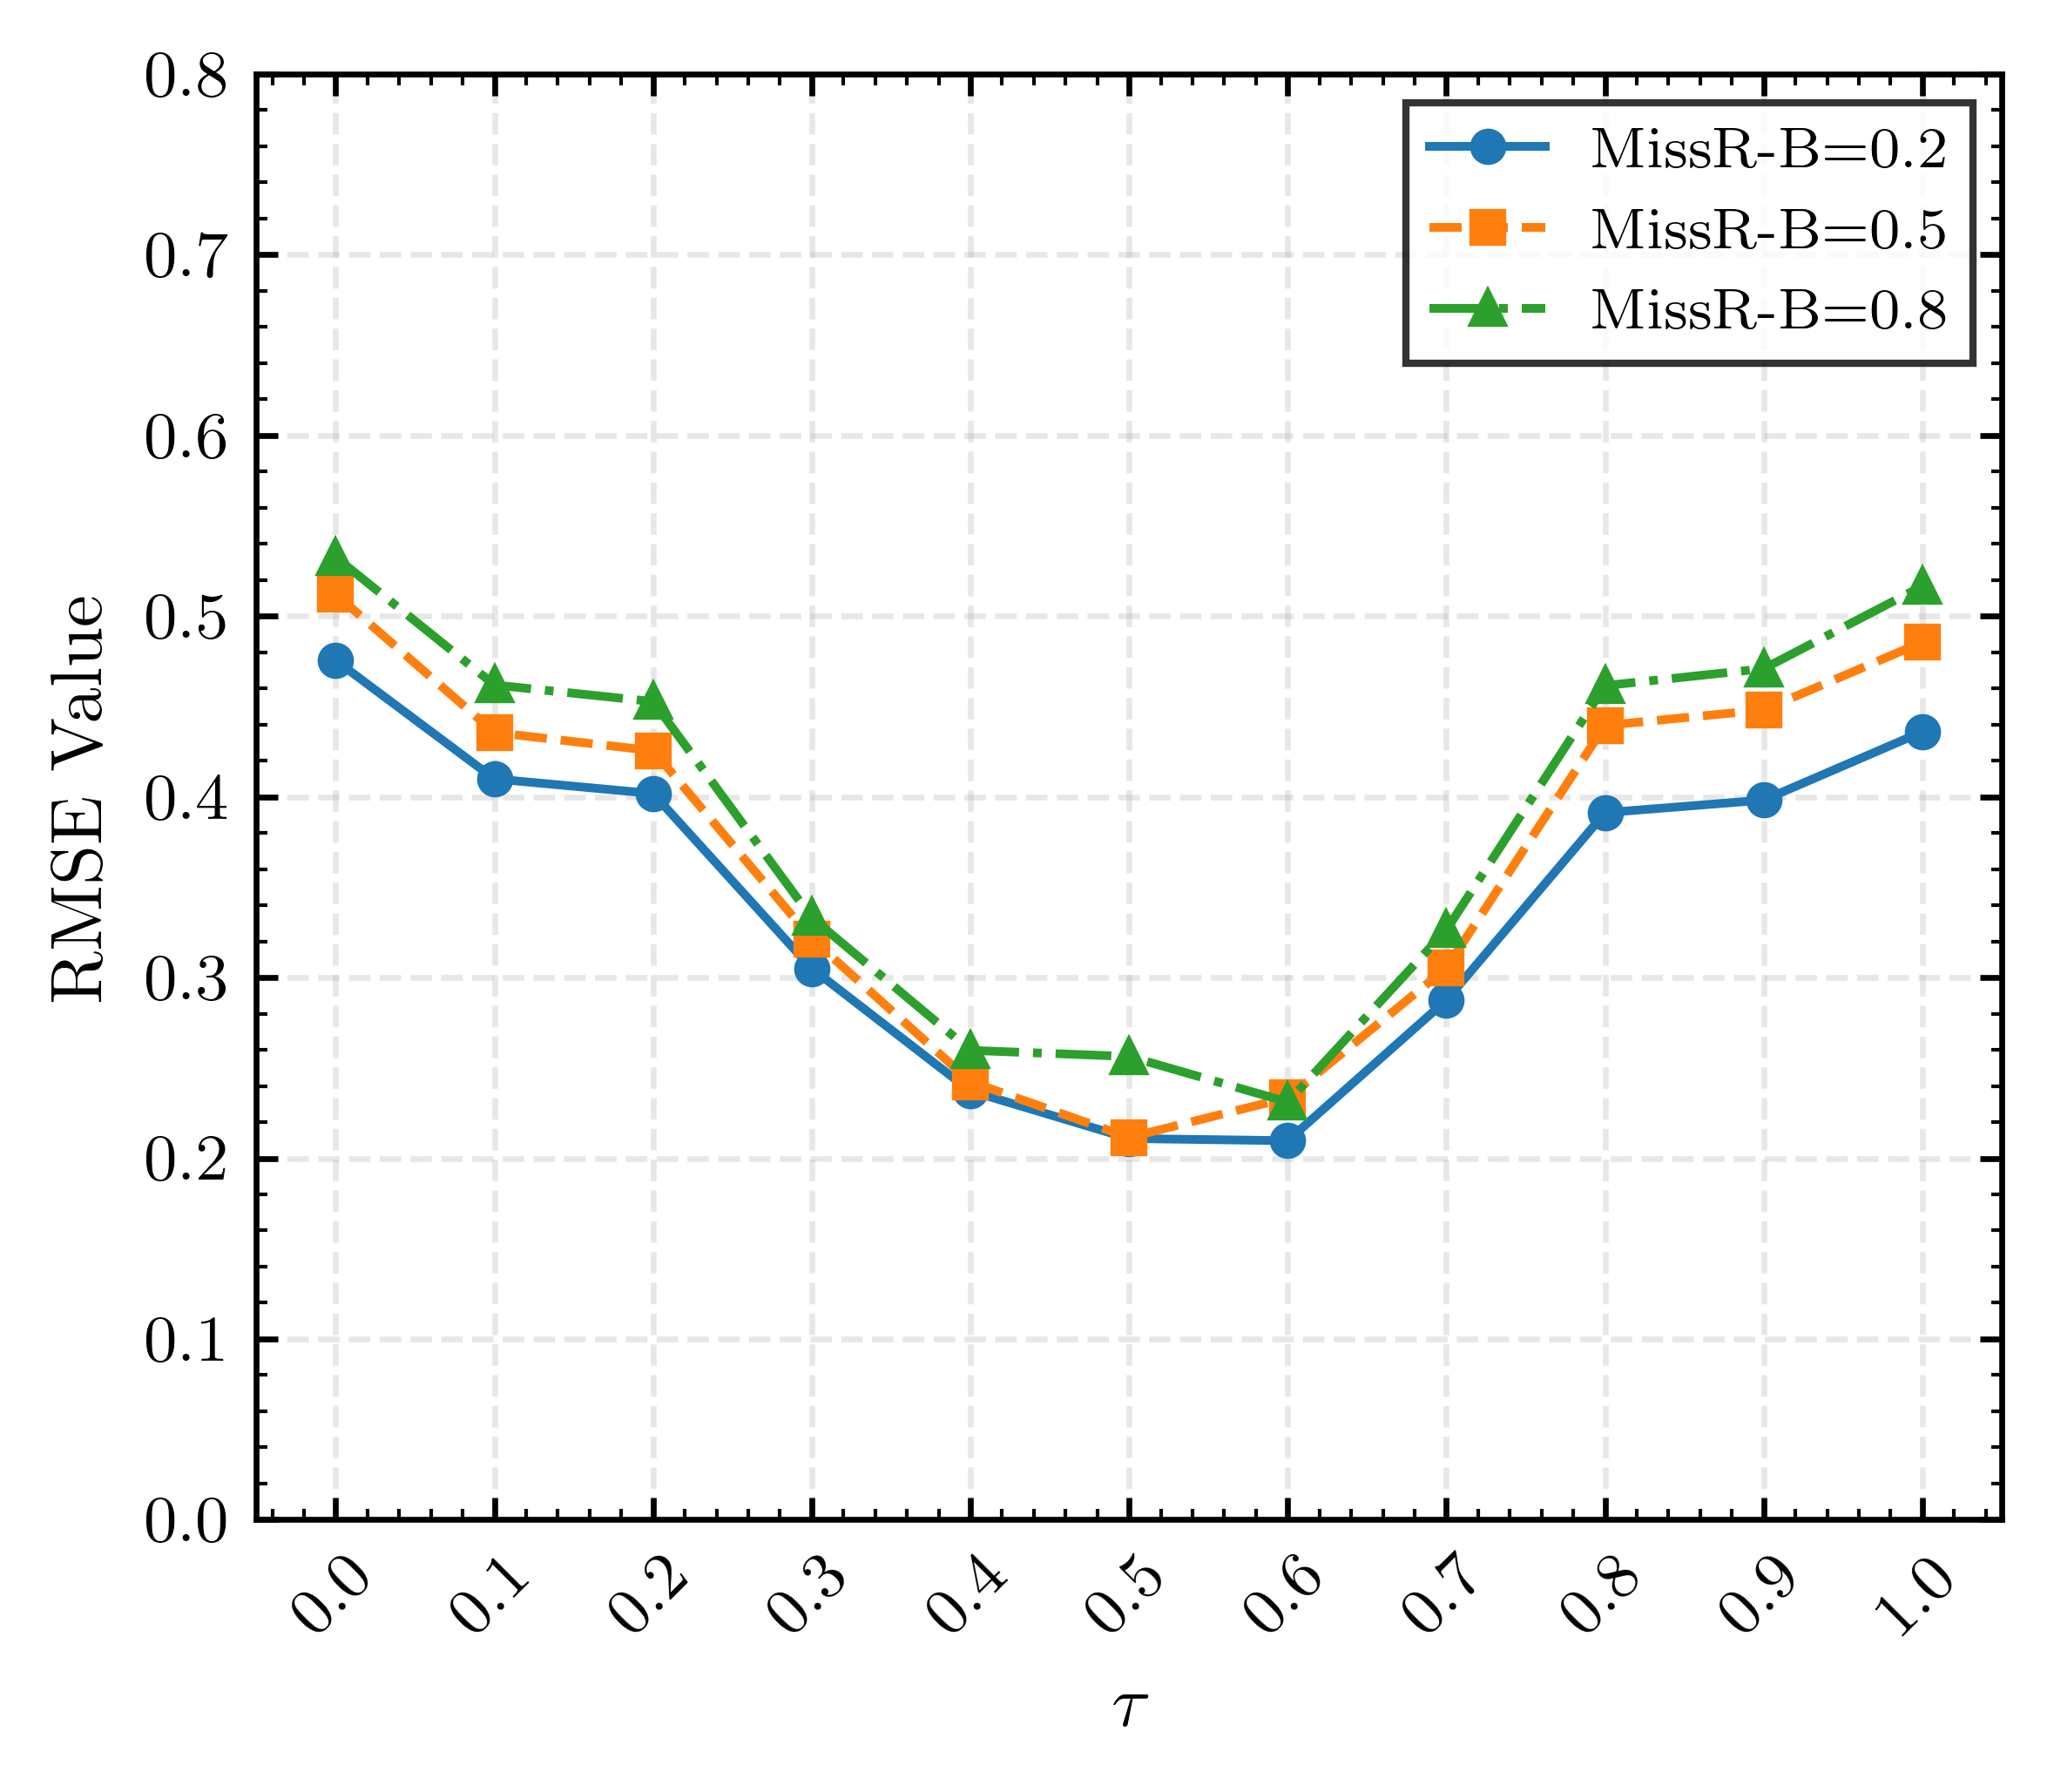
\includegraphics[width=0.45\textwidth]{chapters/imgs/Chapter4Exp1Setting1a}}
	\hspace{0.01\textwidth}  % 适当增加间距
	\subfigure[]{
		\label{Chapter4Exp1Setting1b}
		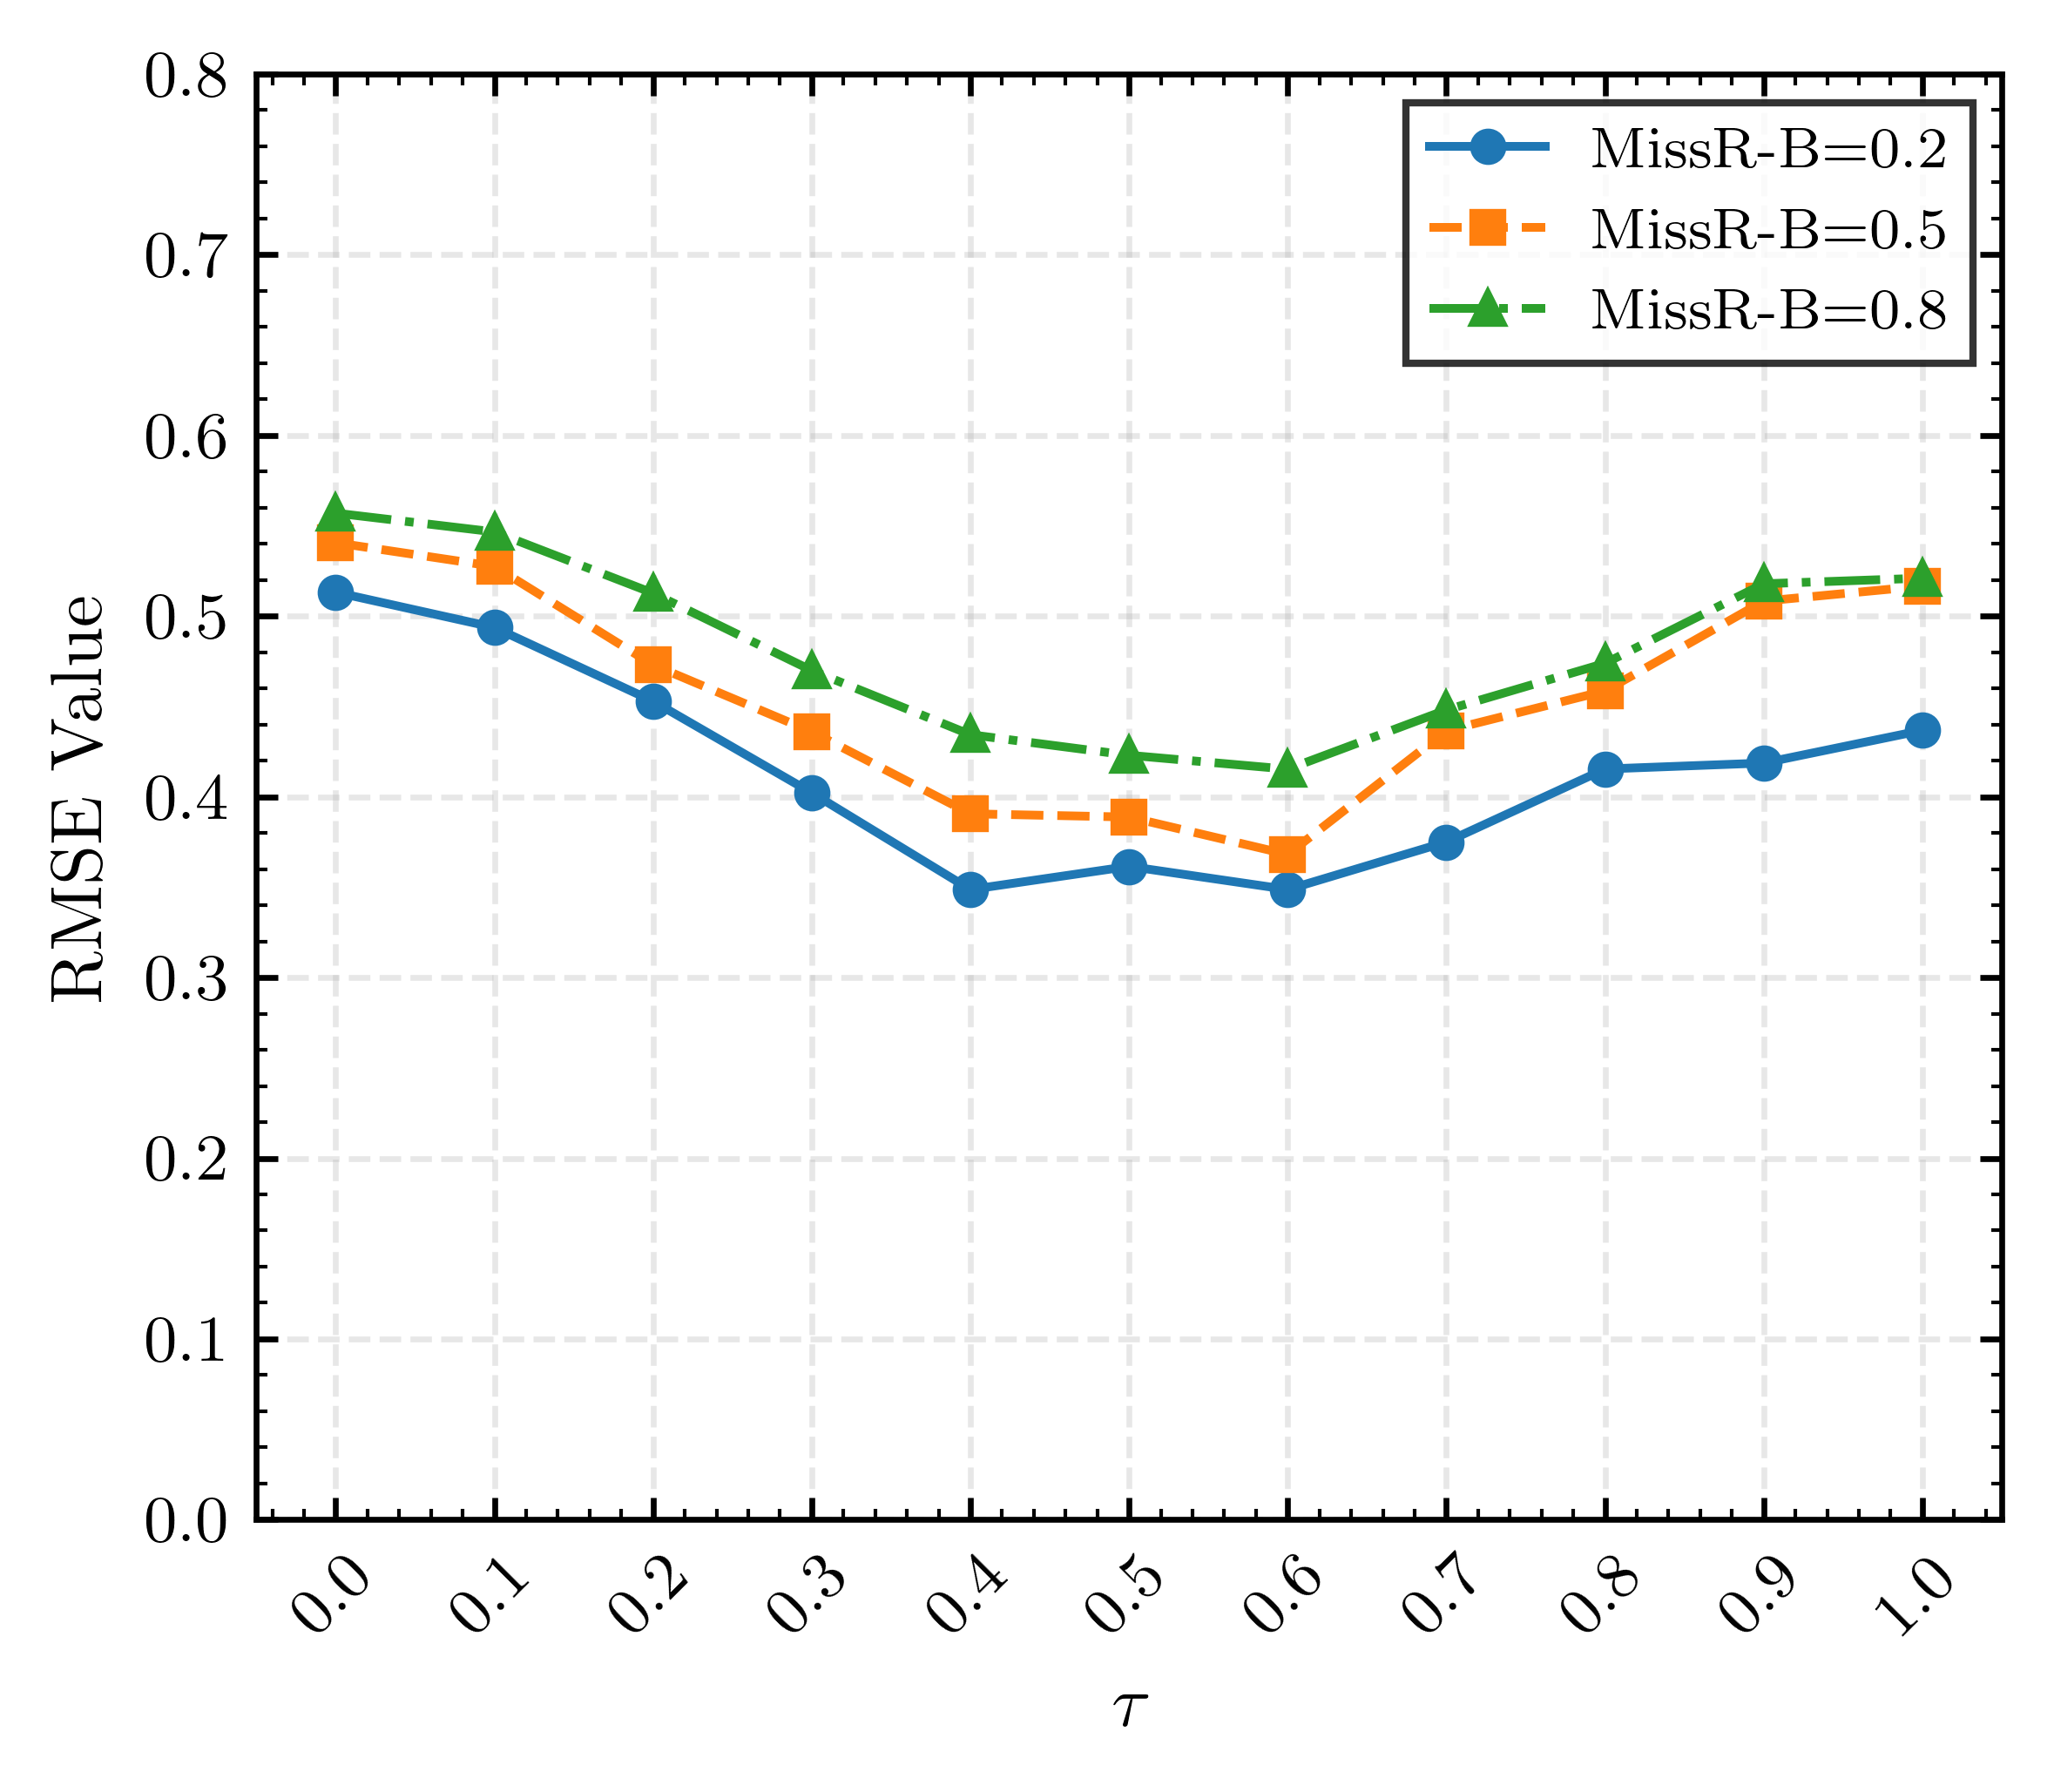
\includegraphics[width=0.45\textwidth]{chapters/imgs/Chapter4Exp1Setting1b}}
	
	\bicaption[\xiaosi \songti 使用 FedPSG-PUM 在不同相关性阈值($\tau$)下获得的 RMSE 线图]%
	{\centering \wuhao FedPSG-PUM 方法在不同缺失率下和不同相关性阈值($\tau$)下的 RMSE 指标 。 (a) Bank数据集;(b) Credit数据集}%
	{\centering \wuhao The RMSE line graph generated using FedPSG-PUM for different correlation thresholds ($\tau$). (a) Bank Dataset; (b) Credit Dataset}    
	\label{Chapter4Exp1Setting1}
\end{figure}
\vspace{-0.35cm}

\vspace{-0.1cm}
\begin{table}[H]
	\centering
	\bicaption[\xiaosi FedPSG-PUG 在 Bank 和 Credit 数据集上使用不同基学习器得到的 RMSE]
	{\wuhao 在 Bank 和 Credit 数据集上 FedPSG-PUM 使用不同基学习器得到的 RMSE}
	{\wuhao  RMSE obtained by FedPSG-PUM with different base estimators for Bank and Credit Dataset}
	\label{Chapter4Exp1Setting2}
	\resizebox{\textwidth}{!}{
		{\wuhao \songti
			\begin{tblr}{
					cell{1}{1} = {c=2}{},
					cell{2}{1} = {r=3}{},
					cell{5}{1} = {r=3}{},
					colspec = {Q[c] Q[c] Q[c] Q[c] Q[c] Q[c]}, % 左对齐+居中
					hline{1,8} = {1.5pt}, % 顶部和底部 1.5pt
					hline{2,5} = {0.75pt} % 中间分隔线 0.75pt
				}
				\diagbox{Datasets \& MisR-B}{Base Estimator} &     & VFPU\_LR & VFPU\_RF & VFPU\_GBDT & VFPU\_LGB \\
				Bank                   & 0.2 & 0.3146   & 0.2640   & 0.2097     & 0.3887    \\
				& 0.5 & 0.3233   & 0.2727   & 0.2335     & 0.3974    \\
				& 0.8 & 0.3400   & 0.2894   & 0.2311     & 0.4141    \\
				Credit                & 0.2 & 0.3596   & 0.3591   & 0.3487     & 0.3666    \\
				& 0.5 & 0.3947   & 0.3942   & 0.3681     & 0.4017    \\
				& 0.8 & 0.4289   & 0.4284   & 0.4153     & 0.4359    
			\end{tblr}
		}
	}
\end{table}
\vspace{-0.4cm}

表 \ref{Chapter4Exp1Setting2} 展示了不同基学习器在固定相关系数阈值$\tau=5$下的性能对比。从实验数据可以观察到,基学习器的选择对FedPSG-PUM方法的预测精度产生了显著影响,且这种影响在不同缺失率环境下表现出一致性。对Bank数据集的分析表明,VFPU\_GBDT在所有缺失率水平(0.2、0.5、0.8)下均表现出明显优势,平均RMSE值比次优模型VFPU\_RF低20.5\%。特别是在低缺失率($\text{MisR-B}=0.2$)条件下,VFPU\_GBDT的RMSE仅为0.2097,较VFPU\_RF(0.2640)降低了20.6\%,较传统VFPU\_LR(0.3146)降低了33.3\%。值得注意的是,随着缺失率提高至0.8,VFPU\_GBDT依然保持了相对稳定的性能(RMSE为0.2311),仅比低缺失率环境下增加了10.2\%。在Credit数据集上,各基学习器之间的性能差异虽然相对减小,但VFPU\_GBDT仍然在所有缺失率条件下取得最优结果。具体而言,当$\text{MisR-B}=0.2$时,VFPU\_GBDT的RMSE为0.3487,相比VFPU\_RF(0.3591)和VFPU\_LR(0.3596)分别降低了2.9\%和3.0\%;当缺失率增至0.5时,这一优势进一步扩大至约6.6\%;在高缺失率(0.8)情况下,VFPU\_GBDT仍保持了约3.0\%的性能优势。综合两个数据集的实验结果,可以得出结论:基于梯度提升决策树的VFPU\_GBDT在不同数据集和各缺失率条件下均表现出最优性能,基于以上分析,确定VFPU\_GBDT作为FedPSG-PUM方法的最优基学习器,并将在后续实验中继续采用该配置。

\vspace{-0.1cm}
\begin{figure}[h]
	\centering
	\subfigure[]{
		\label{Chapter4Exp1Setting3a}
		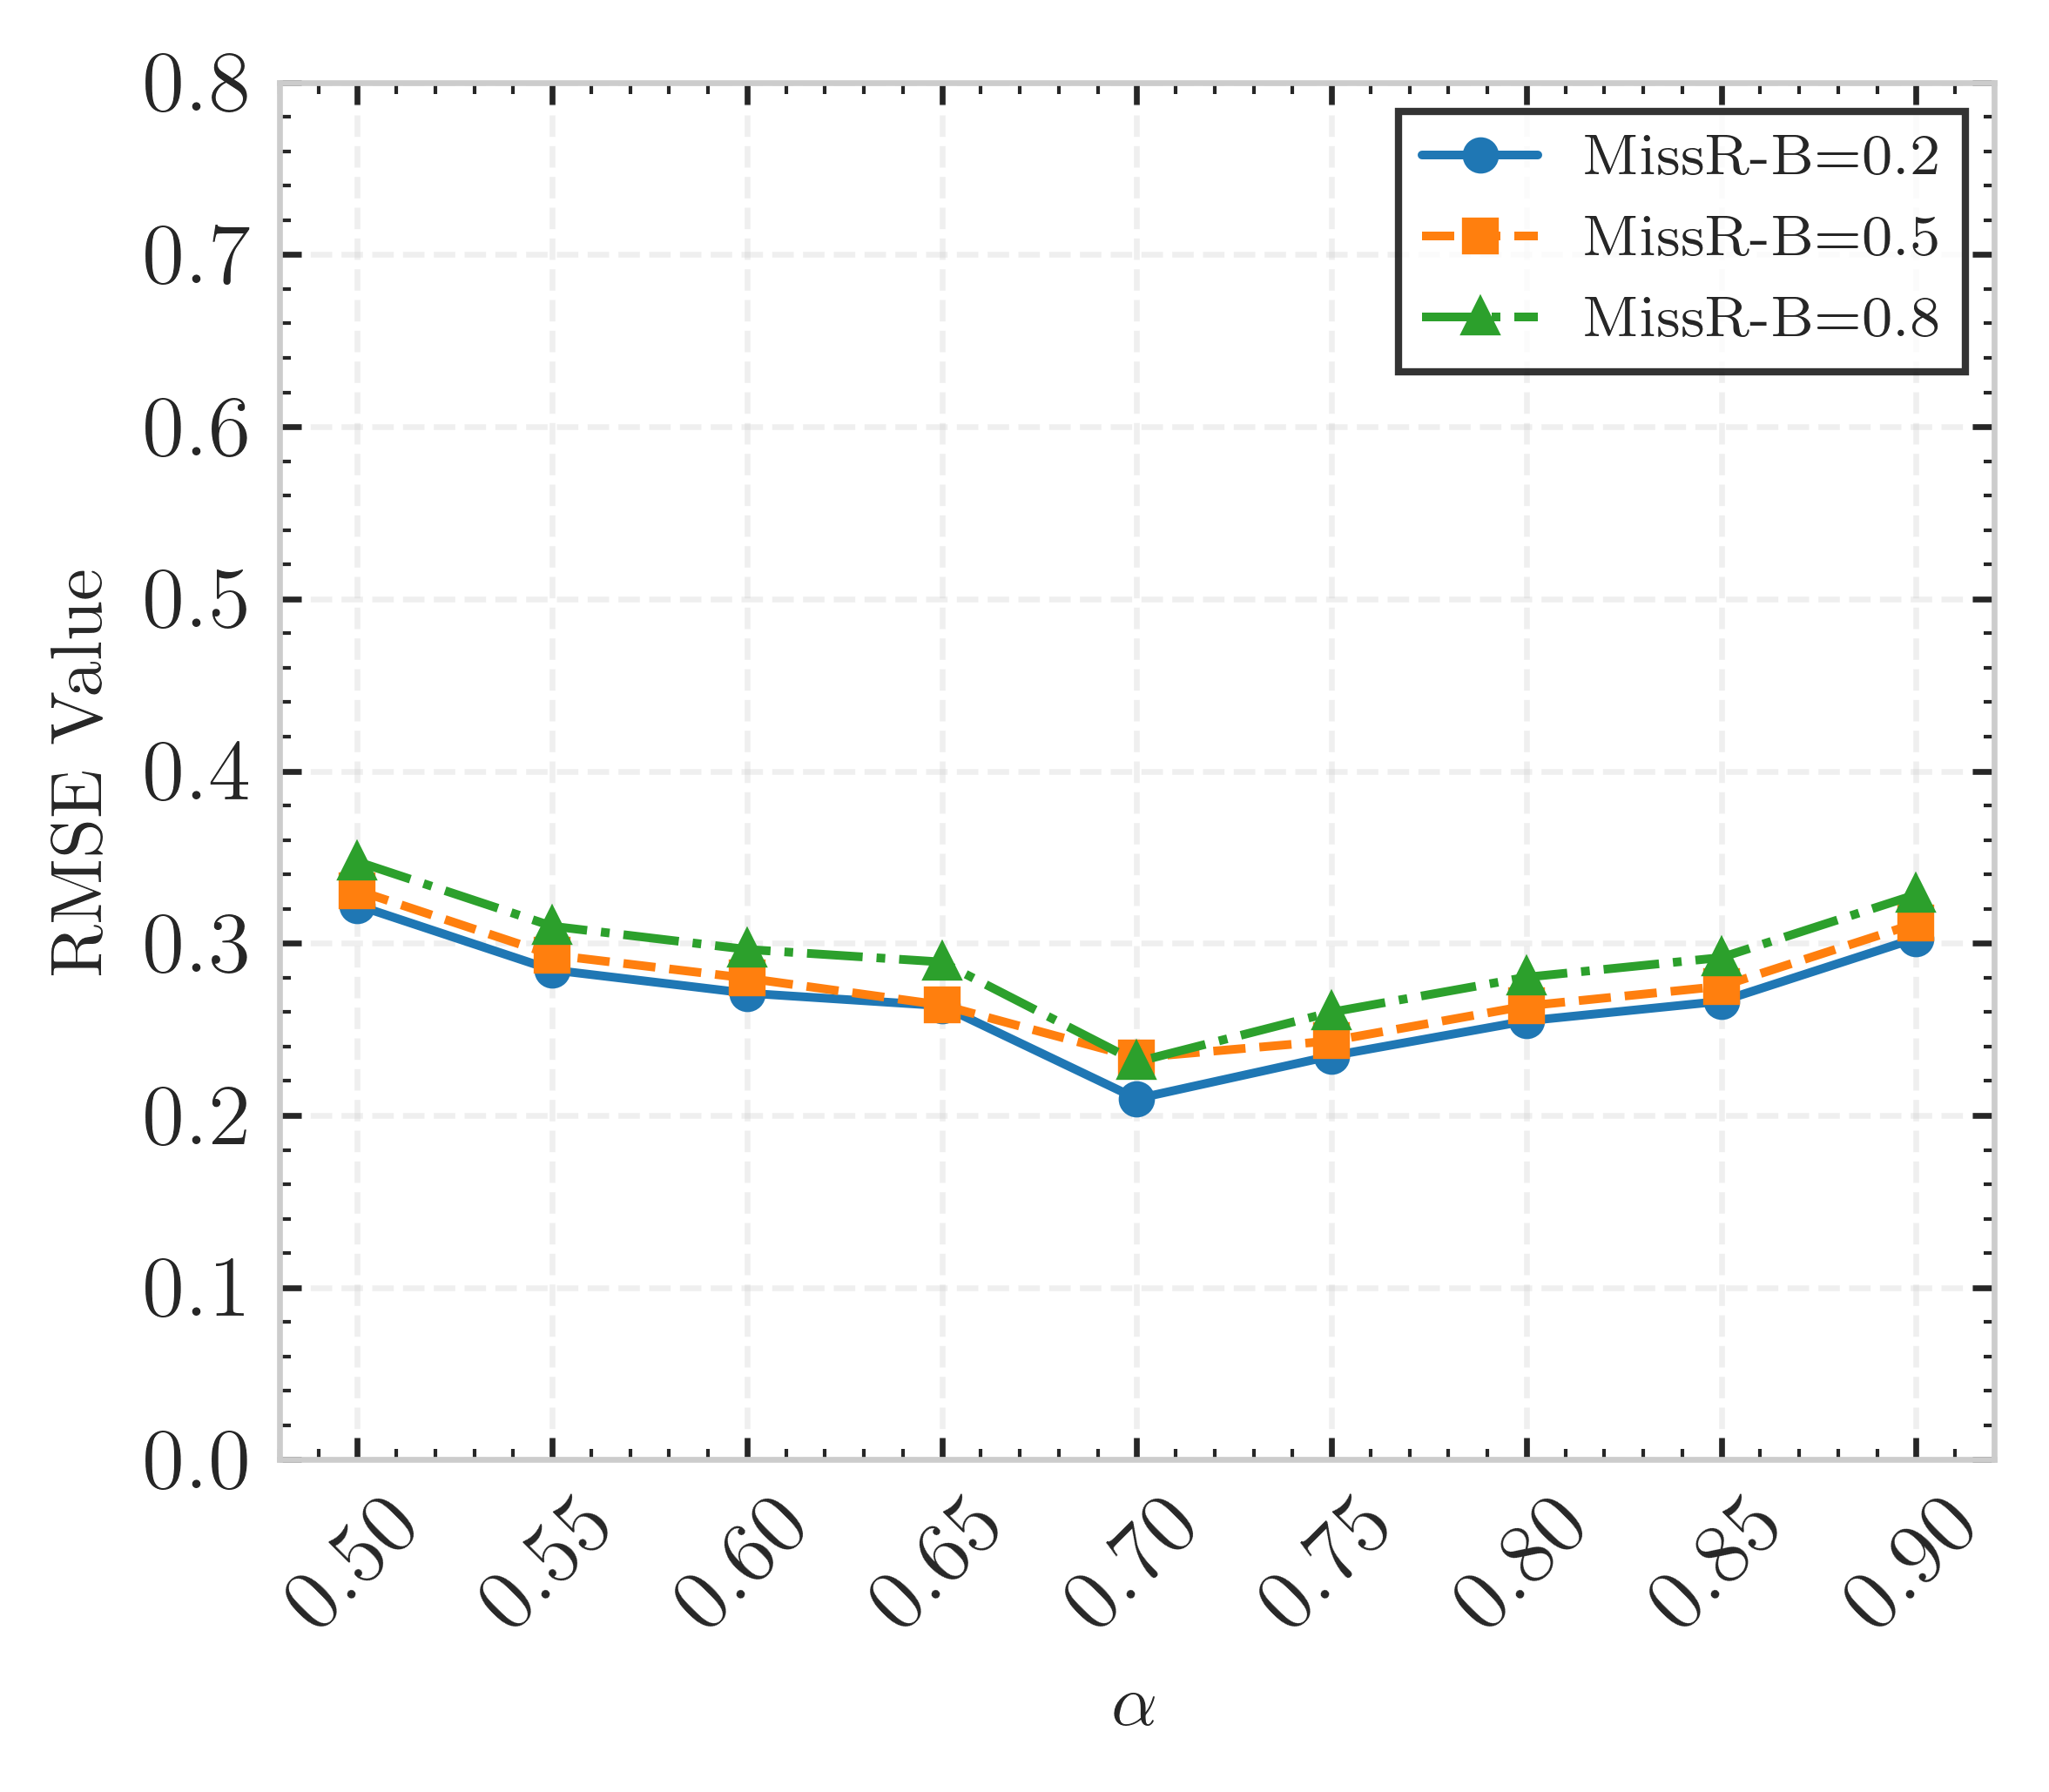
\includegraphics[width=0.45\textwidth]{chapters/imgs/Chapter4Exp1Setting3a}}
	\hspace{0.01\textwidth}  % 适当增加间距
	\subfigure[]{
		\label{Chapter4Exp1Setting3b}
		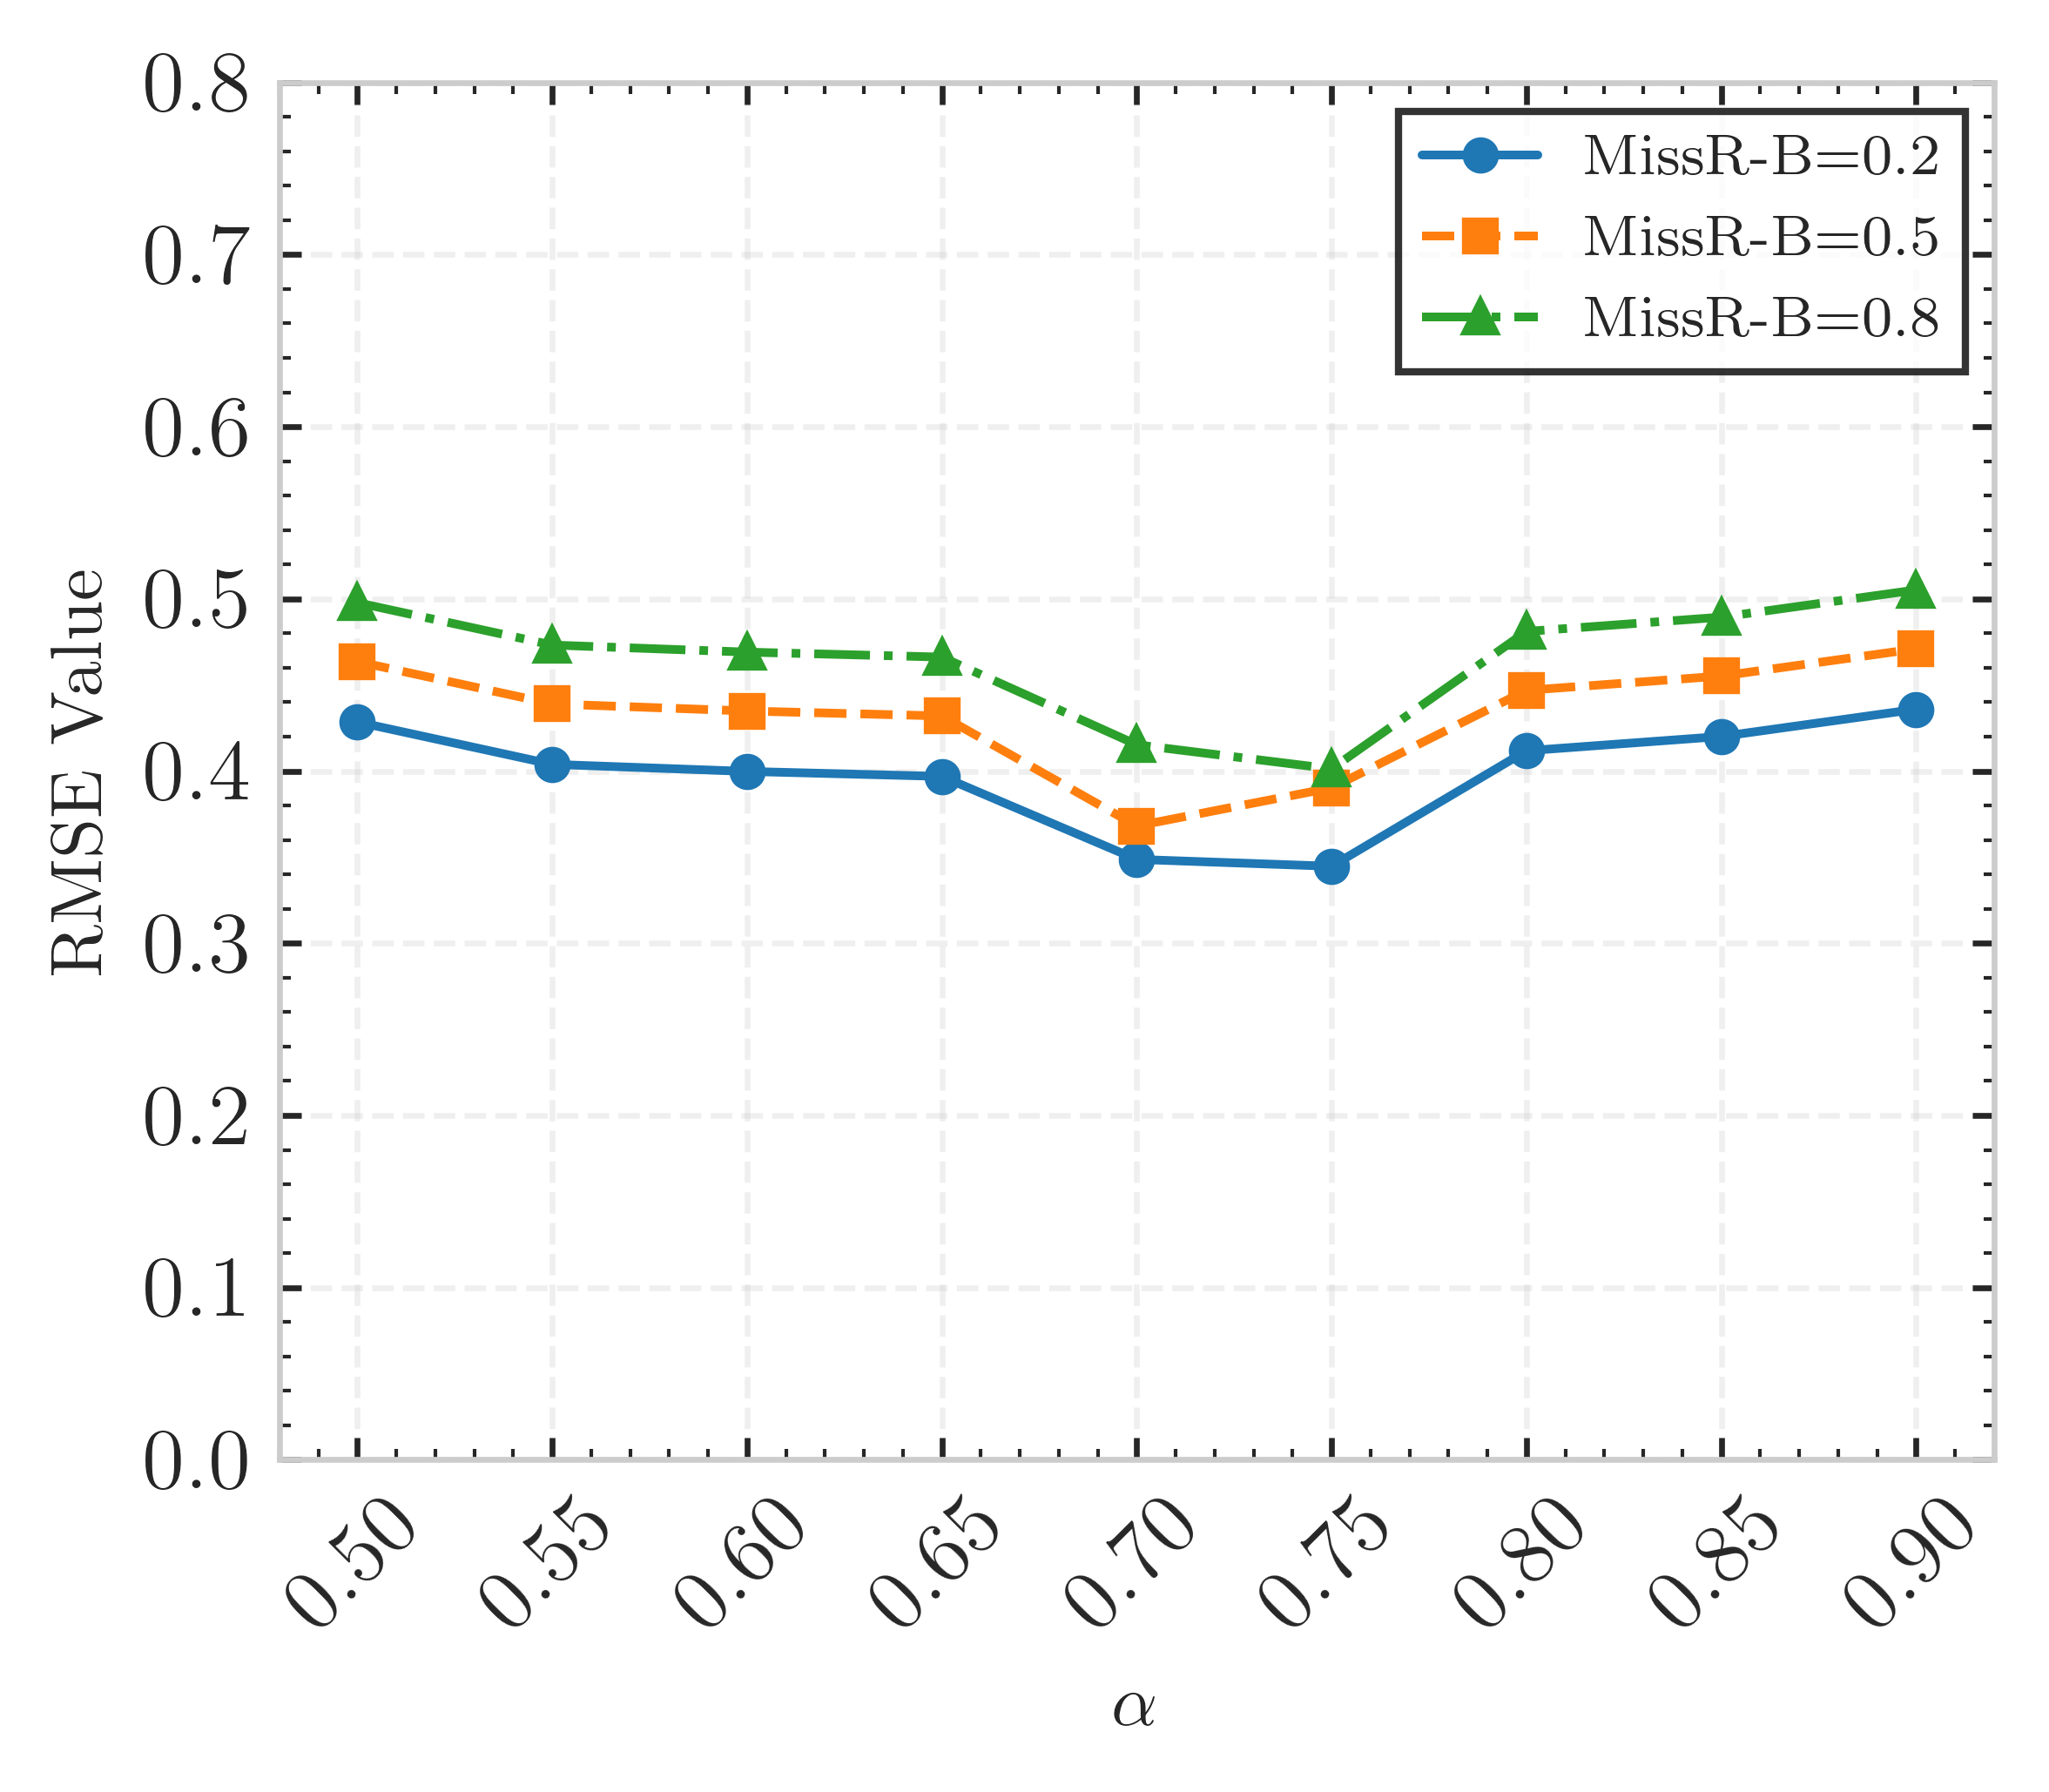
\includegraphics[width=0.45\textwidth]{chapters/imgs/Chapter4Exp1Setting3b}}
	
	\bicaption[\xiaosi \songti 使用 FedPSG-PUM 在不同置信度阈值($\alpha$)下获得的 RMSE 线图]%
	{\centering \wuhao FedPSG-PUM 方法在不同缺失率下和不同置信度阈值($\alpha$)下的 RMSE 指标 。 (a) Bank数据集;(b) Credit数据集}%
	{\centering \wuhao The RMSE line graph generated using FedPSG-PUM for different confidence thresholds ($\alpha$). (a) Bank Dataset; (b) Credit Dataset}    
	\label{Chapter4Exp1Setting3}
\end{figure}
\vspace{-0.35cm}

图 \ref{Chapter4Exp1Setting3} 展示了不同置信度阈值$\alpha$和B方缺失率(MisR-B)组合下的RMSE评估结果。实验结果表明,置信度阈值$\alpha$对模型性能具有一定影响,呈现"U型"的分布特征。随着$\alpha$从0.5逐步提高至0.7,RMSE值持续下降,当$\alpha$超过0.7后,RMSE值开始显著回升。具体而言,在Bank数据集的三种缺失率场景(0.2、0.5和0.8)下,$\alpha=0.7$均产生最优性能,RMSE分别达到0.2097、0.2335和0.2311,较两端端点平均降低约29.8\%的误差。Credit数据集同样呈现相似趋势,在缺失率为0.2和0.5的条件下,$\alpha=0.7$时分别获得0.3487和0.3681的最优RMSE;仅在高缺失率(0.8)场景下,$\alpha=0.75$略优于$\alpha=0.7$,但差异仅为3.4\%。当$\alpha$<0.7时,模型纳入更多低置信度样本扩大训练集规模,但同时引入噪声标签降低学习质量;当$\alpha$>0.7时,筛选条件过于严格,高质量伪标签数量减少,导致模型泛化能力受限。综上所述,实验结果有力支持将置信度阈值$\alpha$设定为0.7,作为FedPSG-PUM框架的最优置信度阈值,并将在后续实验中继续采用该配置。

实验二:基线对比实验,第一组实验在Bank和Credit两个数据集上进行。如表 \ref{Chapter4Exp2Table1} 所示,在单方本地生成模型中,TabDDPM在各缺失率条件下表现最优,其RMSE值分别为Bank数据集(0.4227、0.4728、0.5236)和Credit数据集(0.4478、0.5363、0.575),这验证了扩散模型在表格数据生成任务上的优越性。FedPSG-PUM方法在所有条件下均显著优于单方模型,且性能提升幅度显著。

\vspace{-0.1cm}
\begin{table}[h]
	\centering
	\bicaption[\xiaosi 在Bank和Credit数据集上不同方法在生成B方缺失样本时得到的RMSE]
	{\wuhao 在Bank和Credit数据集上不同方法在生成B方缺失样本时得到的RMSE}
	{\wuhao RMSE of different methods for Party B's missing samples in Bank and Credit datasets}
	\label{Chapter4Exp2Table1}
	\resizebox{\textwidth}{!}{
		{\wuhao \songti
			\begin{tabular}{ccccccc}
				\toprule[1.5pt]
				\multirow{2}{*}{\diagbox{Methods}{Dataset \& MisR-B}} 
				& \multicolumn{3}{c}{Bank} 
				& \multicolumn{3}{c}{Credit} \\
				\cmidrule[0.75pt](lr){2-4} \cmidrule[0.75pt](lr){5-7}
				& 0.2 & 0.5 & 0.8 & 0.2 & 0.5 & 0.8 \\
				\midrule[0.75pt]
				CTGAN           & 0.5099 & 0.5213 & 0.7554 & 0.5456 & 0.6385 & 0.6600 \\
				TableGAN        & 0.5951 & 0.6865 & 0.7312 & 0.6008 & 0.6975 & 0.7838 \\
				CTAB-GAN        & 0.4773 & 0.5644 & 0.6454 & 0.5533 & 0.6674 & 0.6976 \\
				TVAE            & 0.4265 & 0.4862 & 0.6970 & 0.4305 & 0.5534 & 0.6740 \\
				TabDDPM         & 0.4227 & 0.4728 & 0.5236 & 0.4478 & 0.5363 & 0.5750 \\
				FedPSG-PUM(TabDDPM) & 0.2143 & 0.2208 & 0.2436 & 0.3513 & 0.3745 & 0.4353 \\
				FedPSG-PUM(VF-GAIN) & 0.2097 & 0.2115 & 0.2311 & 0.3487 & 0.3681 & 0.4153 \\
				\bottomrule[1.5pt]
			\end{tabular}
		}
	}
\end{table}
\vspace{-0.4cm}

以Bank数据集为例,FedPSG-PUM(VF-GAIN)在MisR-B=0.2时的RMSE仅为0.2097,相比最佳基线模型TabDDPM(0.4227)降低了50.4\%,体现了联邦学习框架在样本生成任务中的显著优势。随着缺失率MisR-B从0.2增加到0.8,所有模型性能均有所下降,但FedPSG-PUM方法的性能降幅明显小于单方模型。例如,在Bank数据集上,TabDDPM的RMSE增加了23.9\%(0.4227→0.5236),而FedPSG-PUM(VF-GAIN)仅增加了10.2\%(0.2097→0.2311)。在FedPSG-PUM框架下,基于VF-GAIN的实现略优于基于TabDDPM的实现,特别是在高缺失率条件下差异更为明显,这表明VF-GAIN在联邦环境中能更有效地捕获数据分布特征。

第二组实验在Letter和News两个数据集上进行,表 \ref{Chapter4Exp2Table2} 显示了在这两个数据集上的RMSE结果。综合来看,单方本地生成方法中TabDDPM依然相对表现优异(如Letter数据集在MisR-B=0.5时可达0.5413;News数据集在MisR-B=0.8时为0.5671),但相比第一组实验,其他生成模型(如TVAE、CTAB-GAN 等)有时在局部指标上也可获得较为接近的性能。联邦协作方式下,FedPSG-PUM(VF-GAIN)和FedPSG-PUM(TabDDPM)再度显现出更为优异的能力,其中FedPSG-PUM(VF-GAIN)在MisR-B=0.2时于Letter数据集得到0.2941的RMSE、在News数据集MisR-B=0.5时取得0.4553,平均而言较单方方法提升幅度超过10\%-20\%。

\vspace{-0.1cm}
\begin{table}[h]
	\centering
	\bicaption
	[\xiaosi 在Letter和News数据集上不同方法在生成B方缺失样本时得到的RMSE]
	{\wuhao 在Letter和News数据集上不同方法在生成B方缺失样本时得到的RMSE}
	{\wuhao RMSE of different methods for Party B's missing samples in Letter and News Dataset}
	\label{Chapter4Exp2Table2}
	\resizebox{\textwidth}{!}{
		{\wuhao \songti
			\begin{tabular}{ccccccc}
				\toprule[1.5pt]
				\multirow{2}{*}{\diagbox{Methods}{Dataset \& MisR-B}} 
				& \multicolumn{3}{c}{Letter} 
				& \multicolumn{3}{c}{News} \\
				\cmidrule[0.75pt](lr){2-4} \cmidrule[0.75pt](lr){5-7}
				& 0.2 & 0.5 & 0.8 & 0.2 & 0.5 & 0.8 \\
				\midrule[0.75pt]
				CTGAN            & 0.5328 & 0.5664 & 0.6218 & 0.5209 & 0.5626 & 0.6034 \\
				TableGAN         & 0.5398 & 0.6148 & 0.7068 & 0.4722 & 0.5204 & 0.6234 \\
				CTAB-GAN        & 0.5226 & 0.5610 & 0.6559 & 0.4815 & 0.5220 & 0.6572 \\
				TVAE            & 0.5203 & 0.5614 & 0.6634 & 0.5018 & 0.5492 & 0.6348 \\
				TabDDPM         & 0.4921 & 0.5413 & 0.5833 & 0.4550 & 0.5024 & 0.5671 \\
				FedPSG-PUM(TabDDPM) & 0.3298 & 0.3674 & 0.3865 & 0.4116 & 0.4492 & 0.4560 \\
				FedPSG-PUM(VF-GAIN) & 0.2941 & 0.3423 & 0.3542 & 0.4333 & 0.4553 & 0.4650 \\
				\bottomrule[1.5pt]
			\end{tabular}
		}
	}
\end{table}
\vspace{-0.4cm}

FedPSG-PUM 的优势在于结合了联邦半监督学习方法和纵向联邦填补方法:利用A方与B方间对齐的样本维度信息,在一定程度上缓解了单方数据不足带来的泛化性能损失;基于联邦半监督VFPU-M算法,对于可信度较高的样本可进行跨方协同训练,从而充分学习潜在的特征分布;VF-GAIN填补模块在补全缺失值时,结合了生成对抗网络与变分推断的优势,进一步提高了缺失数据恢复的精准度。正由于此,FedPSG-PUM(VF-GAIN)与FedPSG-PUM(TabDDPM)在多组实验设置下均呈现较低的RMSE,其中以FedPSG-PUM(VF-GAIN)的平均误差下降幅度更为显著。尤其在高缺失率(MisR-B = 0.8)情形下,FedPSG-PUM(VF-GAIN)在四个数据集的综合RMSE均优于其他方法。

实验三:样本生成效果对比,本实验对FedPSG-CAG、TabDDPM、A∞B-GM和N-GM四种数据处理方法生成的联合样本量进行统计分析,得出以下结论:(1)基于样本生成的FedPSG-CAG、TabDDPM与A∞B-GM三类方法均实现了完整的样本对齐:FedPSG-CAG和TabDDPM通过为B方生成与A方未对齐样本相匹配的补偿数据,使联合样本量达到A方原始样本总量;而A∞B-GM虽然采用VertiGAN生成与B方缺失量相当的合成数据,但由于其生成过程严格遵循A方样本分布特征,最终联合样本量仍由A方数据规模决定。(2)N-GM方法在联合数据集构建过程中表现出显著差异性。该方法采用严格样本对齐机制,当A方样本无法与B方缺失样本形成对应关系时,系统将主动丢弃A方未对齐样本。这种选择性保留机制导致最终联合样本规模受限于B方原始样本基数,因此其构建的联合数据集样本量呈现最小值,显著低于其他三种生成增强方法。

如图 \ref{Chapter4Exp3Bank} 所示,在Bank数据集中,无论B方特征缺失比例如何,采用FedPSG-PUM生成B方缺失样本并构建的联合样本集在所有评估指标(ACC、AUC、F1)上均取得了最佳表现,且这一结果对VF-LR、VF-SVM、VF-GBDT、VF-RF和FinalNet五种纵向联邦分类模型皆适用。与之相比,TabDDPM、A∞B-GM和N-GM三种方法的模型性能依次下降。基于实验结果可从以下两个方面进行分析:

\vspace{-0.1cm}
\begin{figure}[H]
	\centering
	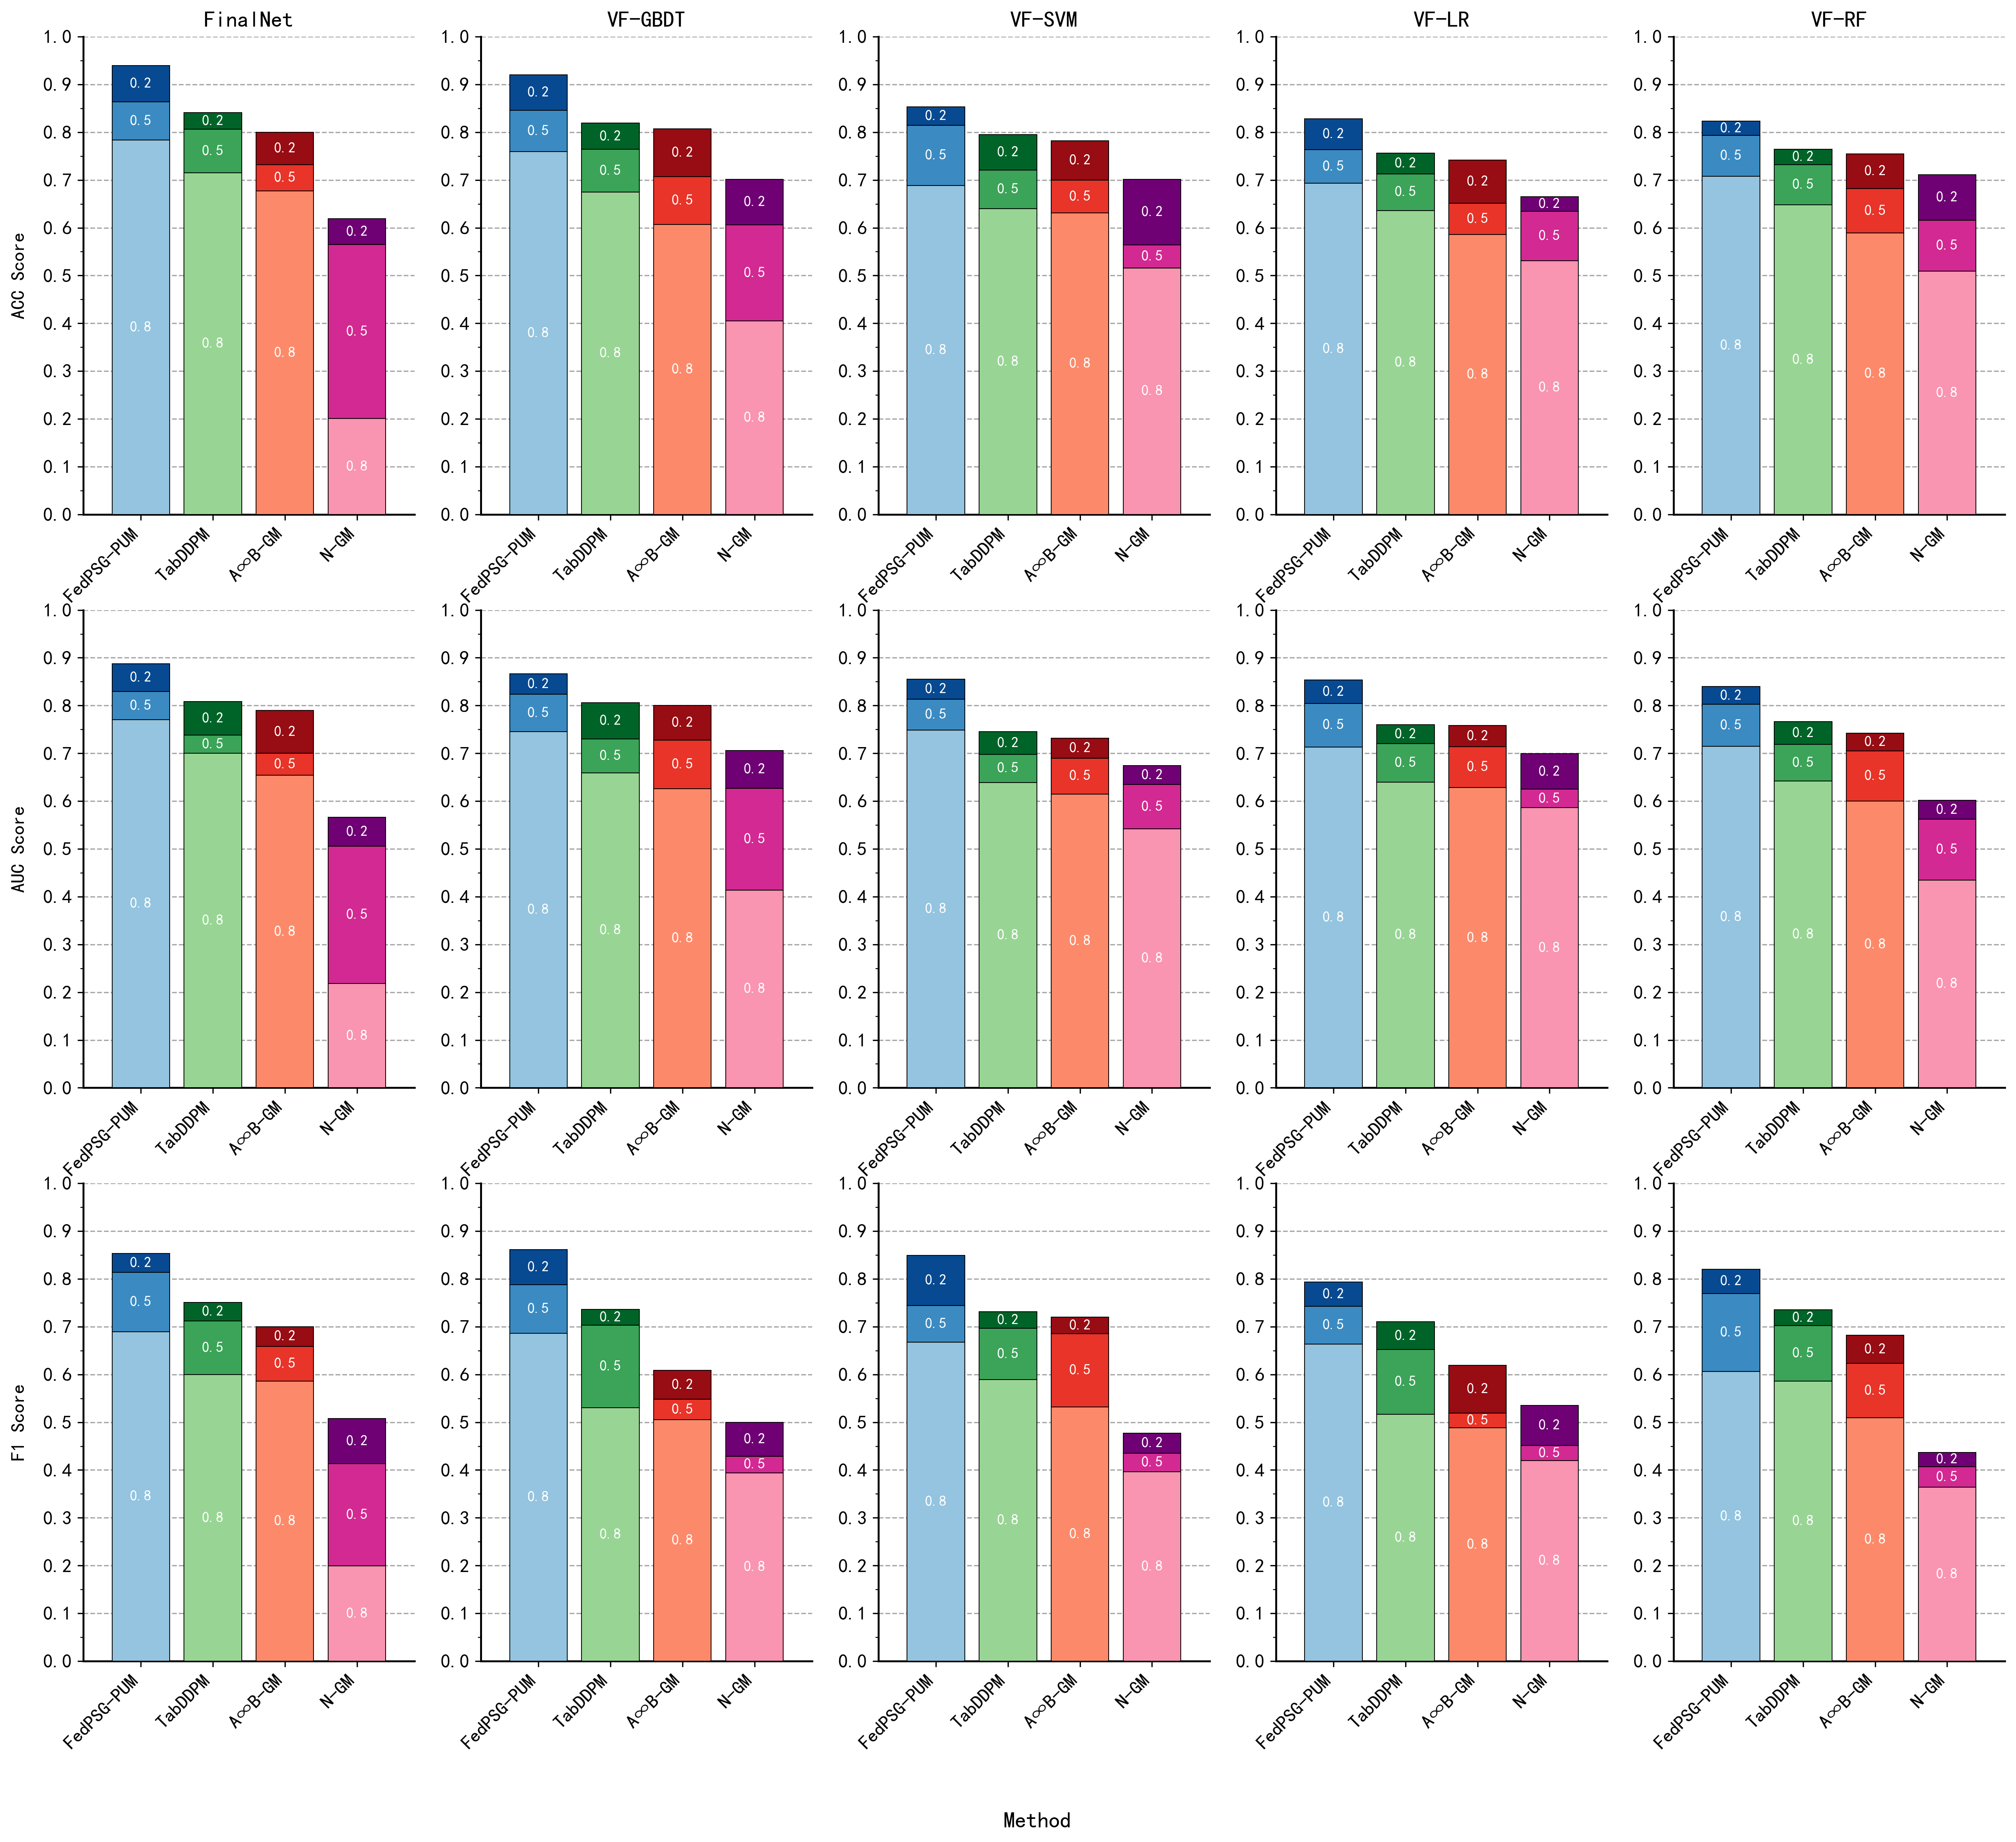
\includegraphics[width=0.9\textwidth]{chapters/imgs/Chapter4Exp3Bank}
	\bicaption[\xiaosi 样本生成效果对比(Bank数据集)]
	{\wuhao 样本生成效果对比(Bank数据集)}
	{\wuhao Sample generation effect comparison (Bank Dataset)}
	\label{Chapter4Exp3Bank}
\end{figure}
\vspace{-0.5cm}

(1)样本数量角度:FedPSG-PUM、TabDDPM与A∞B-GM三种方法均可生成与A方样本数目相当的B方补偿样本,使联合数据集规模相同;而N-GM仅能对齐B方已有样本,导致其最终联合样本量最少。如图 \ref{Chapter4Exp3Bank} 所示,在Bank数据集中,无论缺失比例如何,N-GM构建的联合数据集在各项评估指标上均表现最差。这一结果说明,当其他条件相同的情况下,联合样本量对纵向联邦模型的分类性能具有关键影响。随着B方特征缺失比例上升,N-GM生成的联合样本量急剧下降,导致五种纵向联邦模型的评估指标均明显降低,尤其对于深度神经网络框架FinalNet而言,因其对样本量更加敏感,指标降幅更为显著。这表明在深度学习等复杂模型的纵向联邦训练中,充足的样本量至关重要,而FedPSG-PUM在提升联合样本数量方面具有显著优势。

(2)样本质量角度:尽管FedPSG-PUM、TabDDPM与A∞B-GM这三类方法均实现了与A方数据规模相当的联合样本集,但它们所生成的样本质量存在差异。FedPSG-PUM和TabDDPM均保留了A方的全部真实数据,联合数据中真实样本所占比例较高;而A∞B-GM需要在A方分布的基础上通过VertiGAN生成全新样本,相应地,其联合样本的真实性略逊于前两种方法。进一步而言,FedPSG-PUM不仅能有效学习B方本地高相关属性的分布特征,还可利用多方数据间的关联信息生成更优质的补偿样本,因而在TabDDPM方法之上实现了进一步提升。实验证明,即使在B方高缺失比例条件下,FedPSG-PUM仍能够提供更高质量的训练数据,从而在多种纵向联邦模型中展现更优性能。这也表明纵向联邦学习不仅需要充分的样本数量,还需兼顾样本质量,二者对于模型性能提升同样重要。
\section{本章小结}
本章主要介绍了基于联邦半监督学习的样本参与方生成方法(FedPSG-PUM),旨在有效解决纵向联邦学习中由于样本未对齐导致的特征缺失问题。首先,通过问题分析与定义,明确了纵向联邦学习场景下样本未对齐问题的特征缺失本质,提出了基于联邦半监督学习与表格数据生成相结合的总体解决思路。

接下来,详细阐述了FedPSG-PUM方法的整体框架,包括跨方特征相关性分析、纵向联邦半监督学习预测缺失数据、以及基于生成模型补全低相关性特征等三个主要流程。在跨方特征相关性分析阶段,本章采用了隐私保护下的Spearman秩相关方法,通过同态加密技术保护数据隐私,系统性地计算了跨方特征相关性矩阵。在纵向联邦半监督学习预测阶段,提出了多任务联邦半监督算法VFPU-M,以高效生成高相关性的缺失特征。对于相关性较低的特征,本章引入生成模型(如VF-GAIN和TabDDPM)进一步提高缺失数据生成质量。

在实验验证与分析环节,本章基于UCI机器学习库中四个真实数据集(Bank、Credit、Letter、News)开展了广泛的实验研究与性能评估。实验结果表明,相较于现有方法(如单方生成模型TabDDPM与联邦样本生成方法VertiGAN),FedPSG-PUM在数据生成质量与联合训练模型性能两个方面均表现出明显优势。

%在不同的缺失率条件下,FedPSG-PUM方法构建的联合样本集不仅在数量上满足联邦训练需求,在质量上也更贴近真实数据分布,从而显著提升了纵向联邦分类模型的泛化性能和鲁棒性。

%综上所述,FedPSG-PUM方法通过融合联邦半监督学习与生成模型技术,有效解决了纵向联邦学习场景下的特征缺失问题,实现了非对齐数据的高效利用。实验验证充分证明了其在数据隐私保护前提下的优越性与实用性,为纵向联邦学习框架的进一步研究与应用提供了理论基础和方法支持。